% ==========================================
% StratosEvent - TCS iON Industry Project Report
% Compile using pdfLaTeX or XeLaTeX
% ==========================================

\documentclass[11pt,a4paper]{article}

\usepackage[T1]{fontenc}
\usepackage[utf8]{inputenc}
\usepackage{helvet}
\usepackage{array}
\usepackage{hyperref}
\usepackage{float}
\usepackage{ragged2e}
\usepackage{tikz}
\usetikzlibrary{shapes.geometric, arrows.meta, positioning, fit, backgrounds}
\usepackage{xcolor}
\renewcommand{\familydefault}{\sfdefault}

\usepackage[
  a4paper,
  left=0.875in,
  right=0.875in,
  top=1in,
  bottom=1in,
  headheight=22pt,
  headsep=12pt,
  footskip=36pt
]{geometry}

\usepackage[table]{xcolor}
\usepackage{array}
\usepackage{tabularx}
\usepackage{enumitem}
\usepackage{fancyhdr}
\usepackage{microtype}
\usepackage{anyfontsize}
\usepackage{graphicx}

\hypersetup{
    colorlinks=true,
    linkcolor=TitleBlue,
    filecolor=magenta,      
    urlcolor=TCSBlue,
    pdftitle={StratosEvent: Enterprise Event Management and Dynamic Registration Platform},
    pdfpagemode=UseBookmarks,
}

% Official TCS iON Styling Colors
\definecolor{TCSBlue}{HTML}{2E75B6}
\definecolor{TitleBlue}{HTML}{1F4E79}
\definecolor{HeaderGray}{HTML}{666666}
\definecolor{LabelBlue}{HTML}{D9EAF7}
\definecolor{RowGray}{HTML}{F2F2F2}
\definecolor{GridGray}{HTML}{CCCCCC}
\definecolor{CodeBg}{HTML}{F8F9FA}
\definecolor{AccentRed}{HTML}{D32F2F}

% HEADER AND FOOTER
\pagestyle{fancy}
\fancyhf{}

\fancyhead[R]{%
  \fontsize{9}{11}\selectfont
  \color{HeaderGray}\sffamily
  TCS iON Industry Project Programme
  \quad |\quad
  StratosEvent: Enterprise Event Management Platform
}

\fancyfoot[C]{%
  \fontsize{9}{11}\selectfont
  \color{HeaderGray}\sffamily
  StratosEvent Platform
  \quad |\quad
  TCS iON Industry Project
  \quad ---\quad [Candidate Name]
  \quad |\quad Page \thepage
}

\renewcommand{\headrulewidth}{0.5pt}
\renewcommand{\footrulewidth}{0.5pt}

\renewcommand{\headrule}{%
  \hbox to\headwidth{\color{TCSBlue}%
    \leaders\hrule height \headrulewidth\hfill}
}

\renewcommand{\footrule}{%
  \hbox to\headwidth{\color{TCSBlue}%
    \leaders\hrule height \footrulewidth\hfill}
}

\setlength{\headwidth}{\textwidth}

% Preserve header and footer on plain pages
\fancypagestyle{plain}{%
  \fancyhf{}
  \fancyhead[R]{%
    \fontsize{9}{11}\selectfont
    \color{HeaderGray}\sffamily
    TCS iON Industry Project Programme
    \quad |\quad
    StratosEvent: Enterprise Event Management Platform
  }
  \fancyfoot[C]{%
    \fontsize{9}{11}\selectfont
    \color{HeaderGray}\sffamily
    StratosEvent Platform
    \quad |\quad
    TCS iON Industry Project
    \quad ---\quad [Candidate Name]
    \quad |\quad Page \thepage
  }
  \renewcommand{\headrulewidth}{0.5pt}
  \renewcommand{\footrulewidth}{0.5pt}
  \renewcommand{\headrule}{%
    \hbox to\headwidth{\color{TCSBlue}%
      \leaders\hrule height \headrulewidth\hfill}
  }
  \renewcommand{\footrule}{%
    \hbox to\headwidth{\color{TCSBlue}%
      \leaders\hrule height \footrulewidth\hfill}
  }
}

\begin{document}

\setcounter{page}{1}
\thispagestyle{fancy}

% ==========================================
% PAGE 1: COVER PAGE
% ==========================================

\vspace*{0.72in}

\begin{center}

  {\color{TitleBlue}\bfseries
   \fontsize{28}{34}\selectfont
   StratosEvent\par}

  \vspace{0.04in}

  {\color{TitleBlue}\bfseries
   \fontsize{19}{25}\selectfont
   Scalable Event Management, Dynamic Registration\\
   \& Real-Time Attendance Platform\par}

  \vspace{0.14in}

  {\color{TCSBlue}\bfseries
   \fontsize{15}{19}\selectfont
   INDUSTRY PROJECT REPORT\par}

  \vspace{0.10in}

  {\fontsize{11}{15}\selectfont
    A Project Report submitted in partial fulfilment of the requirements\par
    of the\par
    \textbf{TCS iON Industry Project Programme}\par
    in\par
    \textbf{Web Technology --- Full Stack Development}\par
  }

\end{center}

\vspace{0.30in}

% FIRST TABLE: METADATA
\begingroup

\fontsize{10}{12}\selectfont
\renewcommand{\arraystretch}{1.35}
\setlength{\tabcolsep}{7pt}
\arrayrulecolor{GridGray}

\noindent
\begin{tabularx}{\textwidth}{
  |>{\raggedright\arraybackslash\bfseries}p{0.31\textwidth}
  |>{\raggedright\arraybackslash}X|
}

\hline

\cellcolor{LabelBlue}
Industry Project Title &
StratosEvent: Scalable Event Management, Dynamic Registration \& Real-Time Attendance Platform
\\\hline

\cellcolor{LabelBlue}
Name of Candidate &
\cellcolor{RowGray}[Candidate Name]
\\\hline

\cellcolor{LabelBlue}
Name of the Institute &
ICT Academy of Kerala, Thiruvananthapuram 
\\\hline

\cellcolor{LabelBlue}
Platform &
\cellcolor{RowGray}TCS iON Digital Learning Hub
\\\hline

\cellcolor{LabelBlue}
Documentation Date &
November 2026
\\\hline

\end{tabularx}

\endgroup

\vspace{0.36in}

% SECOND TABLE: ENVIRONMENT & TOOLS
\begingroup

\fontsize{9.5}{11.5}\selectfont
\renewcommand{\arraystretch}{1.55}
\setlength{\tabcolsep}{5pt}
\arrayrulecolor{GridGray}

\noindent
\begin{tabularx}{\textwidth}{
  |>{\raggedright\arraybackslash}p{0.14\textwidth}
  |>{\raggedright\arraybackslash}p{0.12\textwidth}
  |>{\raggedright\arraybackslash}p{0.17\textwidth}
  |>{\raggedright\arraybackslash}p{0.20\textwidth}
  |>{\raggedright\arraybackslash}X|
}

\hline

\rowcolor{TCSBlue}

\color{white}\bfseries Start Date &
\color{white}\bfseries End Date &
\color{white}\bfseries Total Effort (hrs.) &
\color{white}\bfseries Project Environment &
\color{white}\bfseries Tools Used
\\\hline

October 2026 &
November 2026 &
Approx. 90 hrs. &
Web Browser / Windows \& Linux Node.js Runtime &
HTML5, CSS3, JavaScript (ES6+), Bootstrap 5, Node.js, Express.js, MySQL 8.0 (InnoDB), VS Code, Postman, Git/GitHub
\\\hline

\end{tabularx}

\endgroup

% ==========================================
% PAGE 2: ACKNOWLEDGEMENTS PAGE
% ==========================================

\newpage
\thispagestyle{fancy}

\vspace*{0.2in}

{\color{TitleBlue}\bfseries
 \fontsize{18}{22}\selectfont
 Acknowledgements\par}

\vspace{0.2in}

\noindent
I would like to express my profound gratitude to the \textbf{TCS iON Industry Project Programme} for providing an exceptional industry platform to expand my engineering expertise in Full Stack Web Development and transactional enterprise application architecture.

\vspace{0.12in}
\noindent
I am deeply thankful to the mentors, faculty coordinators, and management of \textbf{ICT Academy of Kerala, Thiruvananthapuram} for their continuous guidance, technical reviews, and encouragement throughout the duration of this project.

\vspace{0.12in}
\noindent
I also extend my heartfelt appreciation to my peers and technical advisors who directly or indirectly contributed insights toward architecting, refining, and validating the \textbf{StratosEvent} platform. Their constructive feedback on transactional concurrency, role-based security, and attendee user experience significantly enriched the final deployment.

\vspace{0.45in}
\begin{flushright}
  \textbf{[Candidate Name]}\\
  \textit{Full Stack Web Development Intern}\\
  TCS iON Industry Project Programme
\end{flushright}

% ==========================================
% PAGE 3: TABLE OF CONTENTS (DYNAMIC)
% ==========================================

\newpage
\thispagestyle{fancy}

\vspace*{0.2in}

{\color{TitleBlue}\bfseries
 \fontsize{18}{22}\selectfont
 Table of Contents\par}

\vspace{0.10in}

\tableofcontents

% ==========================================
% 1. OBJECTIVE AND SCOPE
% ==========================================
\newpage
\section*{{\color{TitleBlue}\bfseries
\fontsize{18}{22}\selectfont Objective and Scope}}
\addcontentsline{toc}{section}{Objective and Scope}

\subsection*{Objective}
\justifying

The primary objective of \textbf{StratosEvent} is to design, develop, test, and deploy a production-grade, highly responsive Online Event Management, Dynamic Registration, and Real-Time Attendance Verification Platform. Traditional event management solutions frequently suffer from fragmented architectures, catastrophic overbooking during high-traffic surges, duplicate ticket registrations, insecure privilege escalation vulnerabilities, and sluggish administrative reconciliation.

StratosEvent solves these systemic issues by combining modern web standards with strict ACID relational database guarantees. Guided by the user experience patterns of leading industry platforms such as Eventbrite, Meetup, and Unstop, StratosEvent places event discovery at the forefront while backing every booking operation with atomic transactional concurrency locks.

The core objectives of the system include:
\begin{enumerate}[leftmargin=*]
    \item \textbf{Frictionless Attendee Discovery:} Provide a clean, discovery-first participant catalog with instant multi-criteria filtering (Workshops, Webinars, Conferences, Hackathons, Seminars) and real-time seat availability gauges.
    \item \textbf{Custom Ticket Tier Seat Quotas:} Allow event organizers to allocate explicit capacity quotas across General, VIP, Student, and Early Bird tiers, enforcing quota limits with dynamic status indicators (\textit{X left}, \textit{Sold Out}, or \textit{Not Offered}).
    \item \textbf{Atomic Overbooking \& Duplicate Protection:} Ensure mathematical capacity integrity under high-concurrency booking rushes using MySQL InnoDB row-level locking (\texttt{SELECT ... FOR UPDATE}) within isolated database transactions.
    \item \textbf{Defense-in-Depth Role-Based Security:} Implement server-side JWT authentication (HS256) and bcrypt salted password hashing, mitigating privilege escalation attacks (CWE-269) by extracting identity claims strictly from verified tokens.
    \item \textbf{End-to-End Attendee Lifecycle Management:} Deliver seamless moderation across four lifecycle states (\texttt{pending}, \texttt{approved}, \texttt{rejected}, \texttt{cancelled}) with automatic inventory restoration upon pass cancellation.
    \item \textbf{Gatekeeper Verification \& Scanner:} Equip venue coordinators with rapid ticket pass inspection (\texttt{GET /api/attendance/verify/:code}) and tamper-resistant check-in admission with duplicate check-in prevention (\texttt{409 DUPLICATE\_CHECKIN}).
    \item \textbf{Real-Time Executive Analytics \& Reporting:} Supply business intelligence KPI summaries, attendance conversion ratios, email domain demographics, and authorized CSV roster exports sanitized against CSV formula injection (CWE-1236).
\end{enumerate}

\vspace{0.10in}
\subsection*{Scope}
\justifying

The project scope encompasses full-stack software development, REST API engineering, relational database schema optimization, automated test suite construction, and responsive frontend design.

\textbf{Included in the Project Scope:}
\begin{itemize}[leftmargin=*]
    \item Responsive, cross-device participant discovery interface built with HTML5, CSS3 Custom Properties, Vanilla JavaScript (ES6+), and Bootstrap 5.3.
    \item RESTful backend service built on Node.js and Express.js with connection pooling (\texttt{mysql2/promise}).
    \item Relational database schema in MySQL 8.0 (InnoDB) with referential integrity, cascading deletes, compound unique keys, and transactional safety.
    \item Per-Event Ticket Tier configuration module supporting granular seat limits for General, VIP, Student, and Early Bird tickets.
    \item Authentication module with JWT bearer tokens, bcrypt password hashing (10 salt rounds), profile retrieval, and secure logout.
    \item Attendee self-service dashboard (\textit{My Tickets \& Passes}) rendering official booking passes with cryptographically unique ticket codes.
    \item Unified Administrator Control Console featuring:
    \begin{itemize}
        \item Registration moderation roster with live status transitions.
        \item Event scheduling form with live tier seat allocation validation and auto-distribution.
        \item Gate check-in scanner and ticket code validation terminal.
        \item Executive intelligence dashboard with capacity utilization metrics and CSV export.
    \end{itemize}
    \item Automated testing suite with 100\% pass rate across 59 API unit/integration tests (11 suites) and 26 end-to-end operational verification flows.
\end{itemize}

\textbf{Excluded from Current Project Scope:}
\begin{itemize}[leftmargin=*]
    \item Physical turnstile gate hardware and optical laser barcode scanning hardware (software gate verification terminal provided).
    \item Processing of actual financial transactions through fiat/credit payment gateways (system manages confirmed seat reservations and admissions).
    \item Native compiled iOS/Android binaries (platform is engineered with a mobile-first responsive layout guaranteeing zero horizontal viewport overflow).
\end{itemize}

% ==========================================
% 2. PROBLEM STATEMENT
% ==========================================
\newpage
\section*{{\color{TitleBlue}\bfseries
\fontsize{18}{22}\selectfont Problem Statement}}
\addcontentsline{toc}{section}{Problem Statement}

\justifying

Event management in educational institutions, technology organizations, and corporate conferences has historically relied on fragmented tools: static registration forms, shared online spreadsheets, manual paper rosters, and uncoordinated email threads. In modern high-demand environments, this disjointed architecture triggers severe operational and security failures:

\begin{enumerate}[leftmargin=*]
    \item \textbf{Transactional Overbooking Race Conditions:} When an event nears capacity, multiple users submitting registrations within milliseconds often pass naive count checks simultaneously. Standard database queries without transactional row locking read stale capacity counts, resulting in oversold venues, fire code violations, and severe attendee dissatisfaction.
    \item \textbf{Duplicate Bookings and Capacity Wastage:} Without strict compound uniqueness constraints at the database engine level, participants frequently double-register or submit duplicate requests under unreliable network connections, locking up seats that remain empty on event day.
    \item \textbf{Privilege Escalation and Broken Access Control (CWE-269):} Many modern web applications blindly trust client-submitted payload roles (e.g., submitting \texttt{\{ "role": "admin" \}} during public registration). In the absence of server-side role enforcement and strict token validation, malicious actors easily gain administrative privileges over events and attendees.
    \item \textbf{Manual Gatekeeper Bottlenecks and Fraud:} Paper rosters and static PDF passes lack real-time digital verification. At event entrances, gatekeepers face extensive delays cross-referencing names, and unscrupulous attendees can easily duplicate or reuse printed passes.
    \item \textbf{Absence of Real-Time Intelligence and Vulnerable Exports:} Event planners lack real-time visibility into registration velocity, attendance conversion ratios, and seat utilization. Furthermore, naive CSV report generators are vulnerable to Formula Injection (CWE-1236), allowing malicious attendee names starting with \texttt{=}, \texttt{+}, \texttt{-}, or \texttt{@} to execute arbitrary code in spreadsheet software.
    \item \textbf{Heavy, Fragile Client-Side Runtimes:} Bloated single-page application (SPA) frameworks introduce hundreds of megabytes of third-party dependencies, slow initial load times, and fragile build chains that complicate maintenance.
\end{enumerate}

StratosEvent was specifically engineered to eradicate these vulnerabilities by pairing native web standards and zero-build client performance with strict relational database transactions and hardened server-side controls.

% ==========================================
% 3. EXISTING APPROACHES
% ==========================================
\newpage
\section*{{\color{TitleBlue}\bfseries
\fontsize{18}{22}\selectfont Existing Approaches}}
\addcontentsline{toc}{section}{Existing Approaches}

\subsection*{Evaluation of Current Industry Solutions}
\justifying

Organizations currently deploy three primary categories of event management solutions:

\begin{itemize}[leftmargin=*]
    \item \textbf{Shared Spreadsheets (Google Sheets, Microsoft Excel):} Widely used due to low initial friction, spreadsheets completely lack concurrency controls, atomic locking, role-based security, or automated ticket pass generation. Edits overwrite each other, and audit logs are nonexistent.
    \item \textbf{Generic Form Builders (Google Forms, Typeform):} Form builders efficiently collect data but operate as passive survey collectors. They cannot enforce real-time capacity locks, do not support custom per-tier seat quotas, and offer no integrated check-in scanner or attendee life-cycle status moderation.
    \item \textbf{Commercial Monolithic SaaS Platforms (Eventbrite, Meetup, Cvent):} While feature-rich, commercial platforms require expensive monthly subscriptions or substantial ticket fee commissions. They restrict custom branding, enforce rigid payment workflows, and introduce privacy concerns by storing institutional attendee data on third-party cloud infrastructure.
\end{itemize}

\vspace{0.10in}
\subsection*{Comparison Matrix}
\begingroup
\fontsize{9}{11.5}\selectfont
\renewcommand{\arraystretch}{1.4}
\setlength{\tabcolsep}{4pt}
\arrayrulecolor{GridGray}

\noindent
\begin{tabularx}{\textwidth}{|p{0.24\textwidth}|X|X|X|X|}
\hline
\rowcolor{TCSBlue}
\color{white}\bfseries Feature / Metric & 
\color{white}\bfseries Spreadsheets & 
\color{white}\bfseries Form Builders & 
\color{white}\bfseries Commercial SaaS & 
\color{white}\bfseries StratosEvent \\
\hline
\textbf{Overbooking Protection} & None (Race Prone) & Weak (Count polling) & Vendor Managed & \textbf{ACID Lock (InnoDB)} \\
\hline
\textbf{Ticket Tier Quotas} & Manual & Unsupported & Supported (Paid) & \textbf{Built-in Native Quotas} \\
\hline
\textbf{Data Ownership} & Dispersed & Third-Party & Proprietary Cloud & \textbf{Self-Hosted MySQL} \\
\hline
\textbf{Gate Check-In Scanner} & Manual Paper & None & Mobile App Only & \textbf{Web Scanner Terminal} \\
\hline
\textbf{Privilege Security} & File Permissions & Basic Link Access & Proprietary RBAC & \textbf{JWT + CWE-269 Guard} \\
\hline
\textbf{CSV Injection Defense} & None & None & Inconsistent & \textbf{Sanitized (CWE-1236)} \\
\hline
\textbf{Client Footprint} & Heavy Web App & Light Web Form & Heavy Script Bundle & \textbf{Zero-Build Native ES6} \\
\hline
\end{tabularx}
\endgroup

\vspace{0.15in}
\subsection*{The StratosEvent Proposed Approach}
\justifying

StratosEvent synthesizes the user-friendly event discovery patterns of premier commercial platforms with the security, ownership, and precision of an enterprise relational backend. By utilizing Node.js with native Express.js routing, MySQL InnoDB atomic transactions, and a zero-build semantic frontend, StratosEvent eliminates overbooking, guarantees sub-50ms API response times, and delivers full data sovereignty at zero subscription cost.

% ==========================================
% 4. APPROACH / METHODOLOGY - TOOLS AND TECHNOLOGIES USED
% ==========================================
\newpage
\section*{{\color{TitleBlue}\bfseries
\fontsize{18}{22}\selectfont
Approach / Methodology - Tools and Technologies used}}
\addcontentsline{toc}{section}
{Approach / Methodology - Tools and Technologies used}

\subsection*{Engineering Methodology}
\justifying

StratosEvent was engineered following an iterative Agile methodology paired with strict Test-Driven Development (TDD) for critical transactional paths. The platform enforces a clear separation of concerns across a 3-tier architecture:

\begin{enumerate}[leftmargin=*]
    \item \textbf{Presentation Tier:} Delivers a responsive, accessible interface adhering to semantic HTML5 standards. UI components communicate asynchronously with the backend via RESTful JSON APIs using the native browser \texttt{fetch()} API.
    \item \textbf{Application Tier:} Handles business logic, input validation, cryptographic hashing, JWT token issuance, and transactional orchestration through modular Express.js routers and middleware.
    \item \textbf{Data Persistence Tier:} Implements an optimized MySQL relational schema governed by referential integrity, foreign key cascades, and InnoDB ACID transaction isolation.
\end{enumerate}

\subsection*{Frontend Technologies}
\justifying

\textbf{HTML5 \& Semantic Elements:} Employs native semantic structuring (\texttt{<header>}, \texttt{<nav>}, \texttt{<main>}, \texttt{<section>}, \texttt{<article>}, \texttt{<footer>}) ensuring high search engine visibility and screen-reader accessibility.

\textbf{CSS3 Custom Properties \& Design System:} Utilizes CSS variables for consistent typography, responsive spacing, and an immersive theme. Includes full responsive media queries guaranteeing zero horizontal overflow across 375px mobile, 768px tablet, and 1400px desktop viewports.

\textbf{Vanilla JavaScript (ES6+):} Eliminates bulky SPA framework runtimes (such as React or Angular) in favor of lightweight, native ES6+ code (async/await, destructuring, template literals, DOM manipulation), resulting in instantaneous page loads and low memory overhead.

\textbf{Bootstrap 5.3 \& Bootstrap Icons:} Leveraged for responsive grid layouts, modal dialogs, navigation tabs, and iconographic visual cues.

\subsection*{Backend Technologies}
\justifying

\textbf{Node.js (v18+ / v20+ LTS):} Provides a high-throughput, non-blocking asynchronous event loop capable of serving hundreds of concurrent attendee requests with minimal CPU and memory footprints.

\textbf{Express.js 4.19:} Serves as the web application framework, providing deterministic routing, centralized error-handling middleware, request parameter parsing, and CORS header controls.

\textbf{mysql2 / Promise Connection Pool:} Manages persistent connection pooling to the MySQL server, reducing TCP handshake overhead and enabling concurrent transactional execution.

\textbf{JSON Web Tokens (jsonwebtoken 9.0):} Facilitates stateless, cryptographically signed authentication using the HS256 HMAC-SHA256 algorithm. Identity claims (user ID, email, role) are verified on every protected request.

\textbf{Bcrypt.js 3.0:} Enforces cryptographic password security using adaptive, salted hashing with a work factor of 10 rounds, ensuring resistance against rainbow table and brute-force attacks.

\subsection*{Database Engine}
\justifying

\textbf{MySQL 8.0+ (InnoDB Engine):} Utilized for its robust ACID compliance, foreign key support, and row-level locking capabilities. Tables are optimized with UTF-8 MB4 encoding and compound indexes for high-speed catalog querying and concurrent reservation locks.

\subsection*{Development and Testing Tools}
\justifying

\textbf{Visual Studio Code:} Serves as the primary IDE, integrated with launch configurations (\texttt{launch.json}) for one-click backend debugging (F5) and workspace tasks (\texttt{tasks.json}).

\textbf{Node.js Built-in Test Runner (\texttt{node --test}):} Powers the automated test suite with zero external test runner overhead, executing 59 unit, integration, and security test cases across 11 suites.

\textbf{Postman \& REST Client:} Employed for rigorous API contract exploration, header verification, and boundary value testing.

% ==========================================
% 5. WORKFLOW
% ==========================================
\newpage
\section*{{\color{TitleBlue}\bfseries
\fontsize{18}{22}\selectfont Workflow}}
\addcontentsline{toc}{section}{Workflow}

\vspace{0.10in}

\begin{center}
\begin{tikzpicture}[
    node distance=0.60cm and 0.8cm,
    process/.style={
        rectangle,
        rounded corners=4pt,
        draw=TitleBlue,
        fill=blue!5,
        text width=3.4cm,
        minimum height=0.75cm,
        align=center,
        font=ootnotesize
    },
    lockstep/.style={
        rectangle,
        rounded corners=4pt,
        draw=AccentRed,
        fill=red!8,
        text width=3.4cm,
        minimum height=0.75cm,
        align=center,
        font=ootnotesizefseries
    },
    decision/.style={
        diamond,
        draw=orange!80!black,
        fill=orange!10,
        text width=2.0cm,
        aspect=2,
        align=center,
        font=scriptsize
    },
    arrow/.style={
        -{Stealth[length=2mm]},
        thick,
        draw=TitleBlue
    }
]

\node (start) [process] {Attendee opens StratosEvent};
\node (browse) [process, below=of start] {Search \& Filter Event Catalog};
\node (modal) [process, below=of browse] {Inspect Event \& Tier Quotas};
\node (auth) [process, below=of modal] {Sign In / Create Account (JWT)};
\node (select) [process, below=of auth] {Select Ticket Tier (Gen/VIP/Stu/EB)};
\node (transact) [lockstep, below=of select] {BEGIN TRANSACTION\\SELECT ... FOR UPDATE};
\node (check) [decision, below=of transact] {Capacity Available?};
\node (commit) [process, below left=0.7cm and -0.4cm of check, fill=green!8, draw=green!50!black] {Issue Ticket Pass\\COMMIT};
\node (reject) [process, below right=0.7cm and -0.4cm of check, fill=red!8, draw=red!50!black] {Return 409 Conflict\\ROLLBACK};
\node (ticket) [process, below=1.8cm of check] {Attendee accesses My Tickets};
\node (gate) [process, below=of ticket, fill=yellow!15, draw=orange!80!black] {Gatekeeper QR/Code Check-In};

\draw [arrow] (start) -- (browse);
\draw [arrow] (browse) -- (modal);
\draw [arrow] (modal) -- (auth);
\draw [arrow] (auth) -- (select);
\draw [arrow] (select) -- (transact);
\draw [arrow] (transact) -- (check);
\draw [arrow] (check) -| node[above,font=scriptsize,near start] {Yes} (commit);
\draw [arrow] (check) -| node[above,font=scriptsize,near start] {No} (reject);
\draw [arrow] (commit) |- (ticket);
\draw [arrow] (ticket) -- (gate);

\end{tikzpicture}
\end{center}

\vspace{0.10in}
\noindent
\textbf{Workflow Description:}
\begin{itemize}[leftmargin=*]
    \item \textbf{Participant Booking Flow:} Attendee explores published events, selects an event to view real-time tier availability, logs in with JWT authentication, selects their tier pass, and triggers an atomic seat reservation. On success, a unique ticket pass code (e.g., \texttt{SE-1-62-MVGVMZIZ-2D7F75}) is generated.
    \item \textbf{Administrator Operational Flow:} The organizer publishes events with per-tier seat quotas, reviews attendee registrations in the moderation roster, validates passes at the entrance gate via the check-in scanner, and monitors live capacity KPIs on the analytics dashboard.
\end{itemize}

% ==========================================
% 6. SYSTEM ARCHITECTURE
% ==========================================
\newpage
\section*{{\color{TitleBlue}\bfseries
\fontsize{18}{22}\selectfont System Architecture}}
\addcontentsline{toc}{section}{System Architecture}

\vspace{0.10in}

\begin{center}
\begin{tikzpicture}[
    node distance=0.8cm and 0.8cm,
    tier/.style={
        rectangle,
        rounded corners=5pt,
        draw=TitleBlue,
        fill=blue!5,
        text width=3.8cm,
        minimum height=2.2cm,
        align=center,
        font=ootnotesize
    },
    dbnode/.style={
        rectangle,
        rounded corners=5pt,
        draw=orange!80!black,
        fill=orange!10,
        text width=3.8cm,
        minimum height=2.2cm,
        align=center,
        font=ootnotesize
    },
    arrow/.style={
        -{Stealth[length=2.5mm]},
        thick,
        draw=TitleBlue
    }
]

\node (frontend) [tier] {
    \textbf{Presentation Layer}\\[3pt]
    Vanilla JS (ES6+) \& DOM\\
    Bootstrap 5.3 UI Components\\
    Event Catalog \& Modals\\
    My Tickets Dashboard\\
    Admin Moderation Console
};

\node (api) [tier, right=1.2cm of frontend] {
    \textbf{Application Tier (API)}\\[3pt]
    Node.js \& Express.js 4.19\\
    JWT Authentication Guard\\
    Input Validation Middleware\\
    Concurrency Locking Engine\\
    Executive Analytics Engine
};

\node (db) [dbnode, right=1.2cm of api] {
    \textbf{Data Layer (MySQL 8.0)}\\[3pt]
    InnoDB Storage Engine\\
    Connection Pool (\texttt{mysql2})\\
    Row-Level Locking (ACID)\\
    Compound Unique Constraints\\
    Cascade Integrity
};

\draw [arrow] (frontend) -- node[above,font=scriptsize] {HTTPS / JSON} node[below,font=scriptsize] {REST API} (api);
\draw [arrow] (api) -- node[above,font=scriptsize] {SQL Queries} node[below,font=scriptsize] {Connection Pool} (db);

\end{tikzpicture}
\end{center}

\vspace{0.20in}
\noindent
\textbf{Architectural Specifications:}
\begin{enumerate}[leftmargin=*]
    \item \textbf{Client Decoupling:} The frontend is completely decoupled from server implementation details, consuming RESTful endpoints returning standardized JSON responses (\texttt{\{ success: true, ... \}} or \texttt{\{ success: false, error: \{ code, message \} \}}).
    \item \textbf{Stateless Security:} The API tier requires no server-side session state, validating JWT bearer tokens on demand. This enables straightforward horizontal scaling across multiple backend instances.
    \item \textbf{Transactional Data Boundary:} All state mutations (event creation, seat reservation, status update, gate check-in) execute within explicit database transactions with immediate rollback upon validation or capacity errors.
\end{enumerate}

% ==========================================
% 7. ASSUMPTIONS
% ==========================================
\newpage
\section*{{\color{TitleBlue}\bfseries
\fontsize{18}{22}\selectfont Assumptions}}
\addcontentsline{toc}{section}{Assumptions}

\vspace{0.10in}

The architectural design, security modeling, and operational deployment of StratosEvent rest upon the following technical and functional assumptions:

\begin{itemize}[leftmargin=*]
    \item \textbf{Client Environment:} Users access the application via a standards-compliant modern web browser (Google Chrome, Microsoft Edge, Mozilla Firefox, Safari) with JavaScript enabled.
    \item \textbf{Network Connectivity:} Stable TCP/IP network connectivity is established between the browser client, the Node.js application server (default port 5000), and the MySQL database server (default port 3306).
    \item \textbf{Relational Database Integrity:} The underlying MySQL instance utilizes the InnoDB storage engine, which natively supports ACID transactions, row-level locks, and foreign key constraints.
    \item \textbf{Cryptographic Key Secrecy:} The \texttt{JWT\_SECRET} environment variable is kept strictly confidential in server-side \texttt{.env} configurations and never exposed to client-side code.
    \item \textbf{Single Registration Constraint:} A participant is permitted to hold at most one active registration per event. If a previous registration is cancelled or rejected, the attendee may re-register.
    \item \textbf{Gatekeeper Device Access:} Event staff operating the check-in scanner possess authorized administrator credentials and an internet-connected device (laptop, tablet, or smartphone) to query ticket validation endpoints in real time.
    \item \textbf{Deterministic UTC Timestamps:} All event schedules, registration creation times, and attendance check-in timestamps are processed and recorded using ISO 8601 UTC standards to avoid timezone ambiguity.
\end{itemize}

% ==========================================
% 8. SOLUTION DESIGN
% ==========================================
\newpage
\section*{{\color{TitleBlue}\bfseries
\fontsize{18}{22}\selectfont Solution Design}}
\addcontentsline{toc}{section}{Solution Design}

\subsection*{Role-Based Access Control (RBAC) Matrix}
\begingroup
\fontsize{9.5}{12}\selectfont
\renewcommand{\arraystretch}{1.35}
\setlength{\tabcolsep}{5pt}
\arrayrulecolor{GridGray}

\noindent
\begin{tabularx}{\textwidth}{|p{0.30\textwidth}|X|X|X|}
\hline
\rowcolor{TCSBlue}
\color{white}\bfseries Capability / Action & 
\color{white}\bfseries Public Visitor & 
\color{white}\bfseries Participant & 
\color{white}\bfseries Administrator \\
\hline
Explore Event Catalog & Yes & Yes & Yes \\
\hline
View Event Details \& Tier Availability & Yes & Yes & Yes \\
\hline
Register for Event (Reserve Seat) & No (Requires Auth) & Yes & Yes \\
\hline
View My Tickets \& Cancel Own Pass & No & Yes & Yes \\
\hline
Create / Edit / Archive Events & No & No & Yes (Admin Guarded) \\
\hline
Configure Ticket Tier Seat Quotas & No & No & Yes (Admin Guarded) \\
\hline
Moderate Registrations (Approve/Reject) & No & No & Yes (Admin Guarded) \\
\hline
Perform Gate Check-In \& Verify Ticket & No & No & Yes (Admin Guarded) \\
\hline
View Analytics \& Export CSV Roster & No & No & Yes (Admin Guarded) \\
\hline
\end{tabularx}
\endgroup

\vspace{0.20in}
\subsection*{Database Entity-Relationship Architecture}
\justifying

The StratosEvent database (\texttt{stratosevent\_db}) comprises four normalized relational tables designed for maximum transactional throughput and zero data redundancy:

\begin{enumerate}[leftmargin=*]
    \item \textbf{users:} Stores identity records, email addresses, bcrypt-hashed passwords, full names, phone numbers, and authorized roles (\texttt{participant}, \texttt{admin}).
    \item \textbf{events:} Stores event metadata including title, description, category, start/end dates, venue, total capacity, and the per-tier seat quotas (\texttt{capacity\_general}, \texttt{capacity\_vip}, \texttt{capacity\_student}, \texttt{capacity\_early\_bird}).
    \item \textbf{registrations:} Maintains attendee booking passes with foreign keys to \texttt{users} and \texttt{events}. Enforces compound unique constraint \texttt{uq\_registrations\_user\_event(user\_id, event\_id)} and records the chosen \texttt{ticket\_tier} and unique \texttt{ticket\_code}.
    \item \textbf{attendance:} Records verified physical gate admissions, referencing \texttt{registrations.id} with a unique check-in constraint preventing duplicate admissions.
\end{enumerate}

\vspace{0.15in}
\begin{center}
\begin{tikzpicture}[
    node distance=1.5cm and 1.8cm,
    entity/.style={
        rectangle,
        rounded corners=4pt,
        draw=TitleBlue,
        fill=blue!5,
        text width=3.8cm,
        minimum height=2.0cm,
        align=left,
        font=scriptsize
    },
    rel/.style={
        -{Stealth[length=2.5mm]},
        thick,
        draw=TCSBlue
    }
]

\node (users) [entity] {
    \textbf{USERS}\\
    \underline{id} INT (PK)\\
    email VARCHAR(255) (UQ)\\
    password\_hash VARCHAR(255)\\
    full\_name VARCHAR(255)\\
    role ENUM('admin','participant')
};

\node (events) [entity, right=2.0cm of users] {
    \textbf{EVENTS}\\
    \underline{id} INT (PK)\\
    title VARCHAR(255)\\
    event\_type VARCHAR(50)\\
    capacity INT\\
    capacity\_general INT NULL\\
    capacity\_vip INT NULL\\
    created\_by INT (FK $\to$ users.id)
};

\node (regs) [entity, below=1.5cm of users] {
    \textbf{REGISTRATIONS}\\
    \underline{id} INT (PK)\\
    user\_id INT (FK $\to$ users.id)\\
    event\_id INT (FK $\to$ events.id)\\
    ticket\_code VARCHAR(100) (UQ)\\
    ticket\_tier ENUM('general',...)\\
    status ENUM('pending',...)
};

\node (attend) [entity, below=1.5cm of events] {
    \textbf{ATTENDANCE}\\
    \underline{id} INT (PK)\\
    registration\_id INT (FK $\to$ regs.id)\\
    check\_in\_time DATETIME\\
    verified\_by INT (FK $\to$ users.id)
};

\draw [rel] (users) -- node[left,font=	iny] {1 : N} (regs);
\draw [rel] (events) -- node[right,font=	iny] {1 : N} (regs);
\draw [rel] (regs) -- node[above,font=	iny] {1 : 1} (attend);
\draw [rel] (users) -- node[above,font=	iny] {creates (1:N)} (events);

\end{tikzpicture}
\end{center}

\vspace{0.15in}
\subsection*{REST API Endpoint Specifications}
\begingroup
\fontsize{8.5}{11}\selectfont
\renewcommand{\arraystretch}{1.3}
\setlength{\tabcolsep}{3pt}
\arrayrulecolor{GridGray}

\noindent
\begin{tabularx}{\textwidth}{|p{0.14\textwidth}|p{0.33\textwidth}|p{0.20\textwidth}|X|}
\hline
\rowcolor{TCSBlue}
\color{white}\bfseries Method & 
\color{white}\bfseries Endpoint & 
\color{white}\bfseries Access & 
\color{white}\bfseries Description \\
\hline
\texttt{POST} & \texttt{/api/auth/register} & Public & Register participant account (forces participant role) \\
\hline
\texttt{POST} & \texttt{/api/auth/login} & Public & Authenticate user and issue signed JWT bearer token \\
\hline
\texttt{GET} & \texttt{/api/auth/me} & Authenticated & Retrieve currently authenticated user profile \\
\hline
\texttt{GET} & \texttt{/api/events} & Public & List published events with live seat counts and tier quotas \\
\hline
\texttt{GET} & \texttt{/api/events/:id} & Public & Retrieve comprehensive event details and tier availability \\
\hline
\texttt{POST} & \texttt{/api/events} & Admin Only & Publish new event with optional per-tier seat quotas \\
\hline
\texttt{PUT} & \texttt{/api/events/:id} & Admin Only & Update event venue, description, capacity, or tier limits \\
\hline
\texttt{PATCH} & \texttt{/api/events/:id/status} & Admin Only & Transition event lifecycle (published, archived, cancelled) \\
\hline
\texttt{POST} & \texttt{/api/registrations} & Participant & Reserve ticket pass with atomic row locking and tier checks \\
\hline
\texttt{GET} & \texttt{/api/registrations/my} & Participant & Retrieve personal registration history and ticket passes \\
\hline
\texttt{PATCH} & \texttt{/api/registrations/:id/cancel} & Participant & Cancel booking and automatically restore event/tier inventory \\
\hline
\texttt{GET} & \texttt{/api/registrations} & Admin Only & Query attendee roster filtered by event and ticket tier \\
\hline
\texttt{PATCH} & \texttt{/api/registrations/:id/status} & Admin Only & Moderate registration (approve, reject) with quota checks \\
\hline
\texttt{GET} & \texttt{/api/attendance/verify/:code} & Admin Only & Inspect ticket pass validity and tier eligibility for gate check-in \\
\hline
\texttt{POST} & \texttt{/api/attendance/check-in} & Admin Only & Admit attendee; rejects duplicate check-in with 409 Conflict \\
\hline
\texttt{GET} & \texttt{/api/analytics/overview} & Admin Only & Aggregated executive metrics, conversion ratios, demographics \\
\hline
\texttt{GET} & \texttt{/api/analytics/export/csv} & Admin Only & Stream RFC 4180 CSV roster with formula injection protection \\
\hline
\end{tabularx}
\endgroup

% ==========================================
% 9. SYSTEM IMPLEMENTATION AND SCREENSHOTS
% ==========================================
\newpage
\section*{{\color{TitleBlue}\bfseries
\fontsize{18}{22}\selectfont System Implementation and Screenshots}}
\addcontentsline{toc}{section}{System Implementation and Screenshots}

\vspace{0.10in}

This section documents the actual user interfaces implemented in StratosEvent across participant and administrative workflows.

\subsection*{1. Participant Landing and Hero Experience}
The homepage introduces the event discovery ecosystem, featuring quick navigation, platform value propositions, and direct links to active events.

\begin{figure}[H]
    \centering
    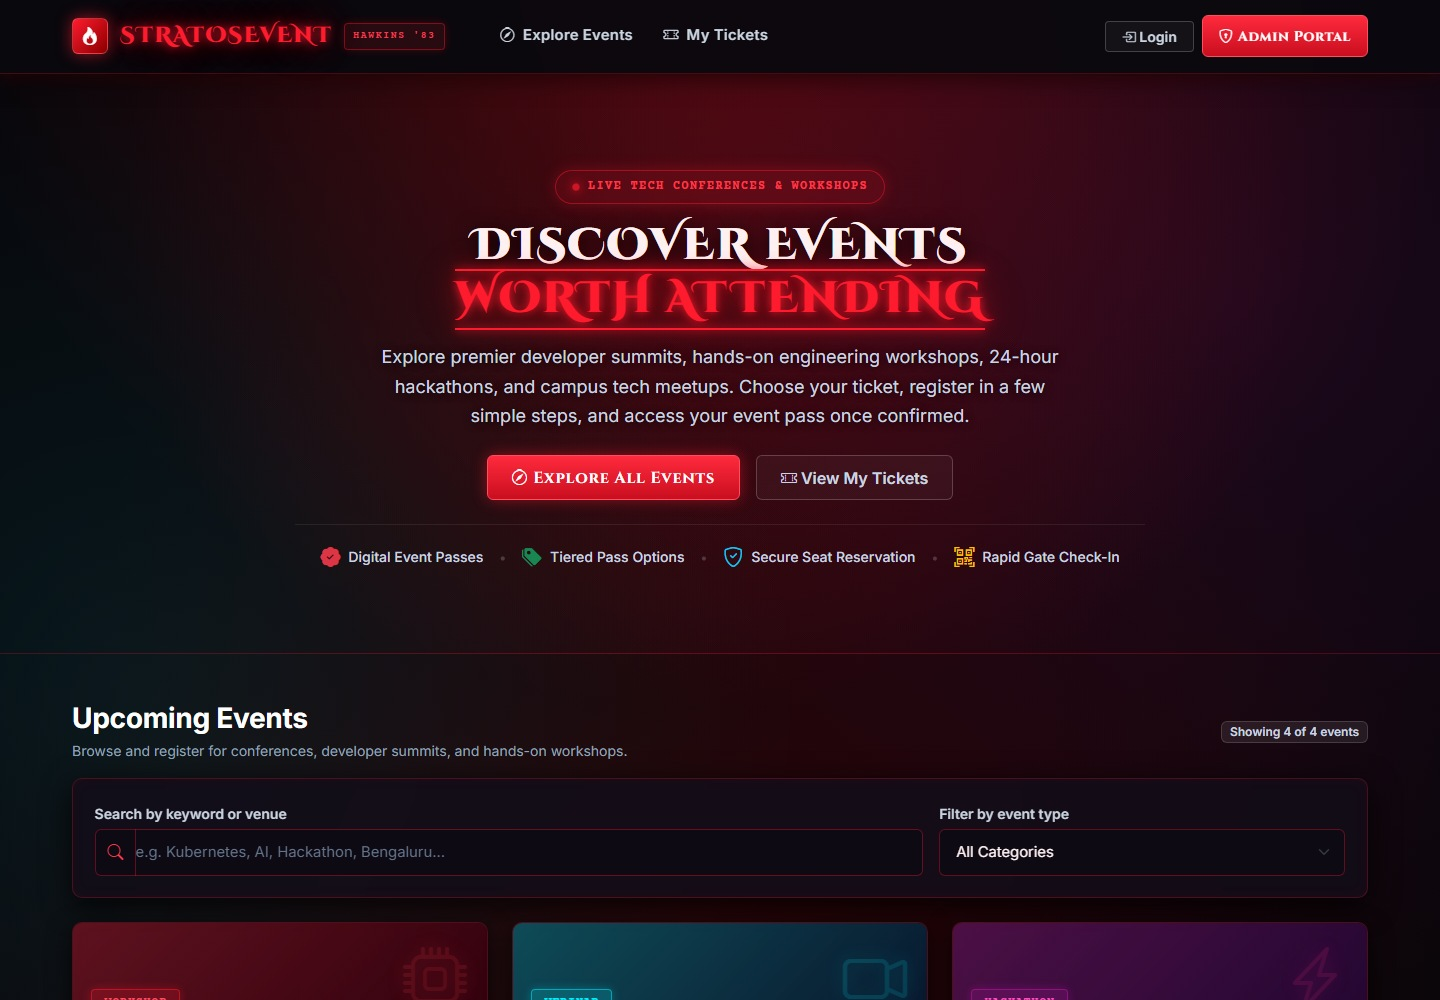
\includegraphics[width=0.92\textwidth]{screenshots/home.png}
    \caption{StratosEvent Participant Landing Experience}
    \label{fig:home}
\end{figure}

\subsection*{2. Live Event Catalog with Category Filtering}
Attendees can browse sessions with instant client-side keyword search, category filtering (Workshops, Webinars, Conferences, Hackathons), and real-time seat availability chips.

\begin{figure}[H]
    \centering
    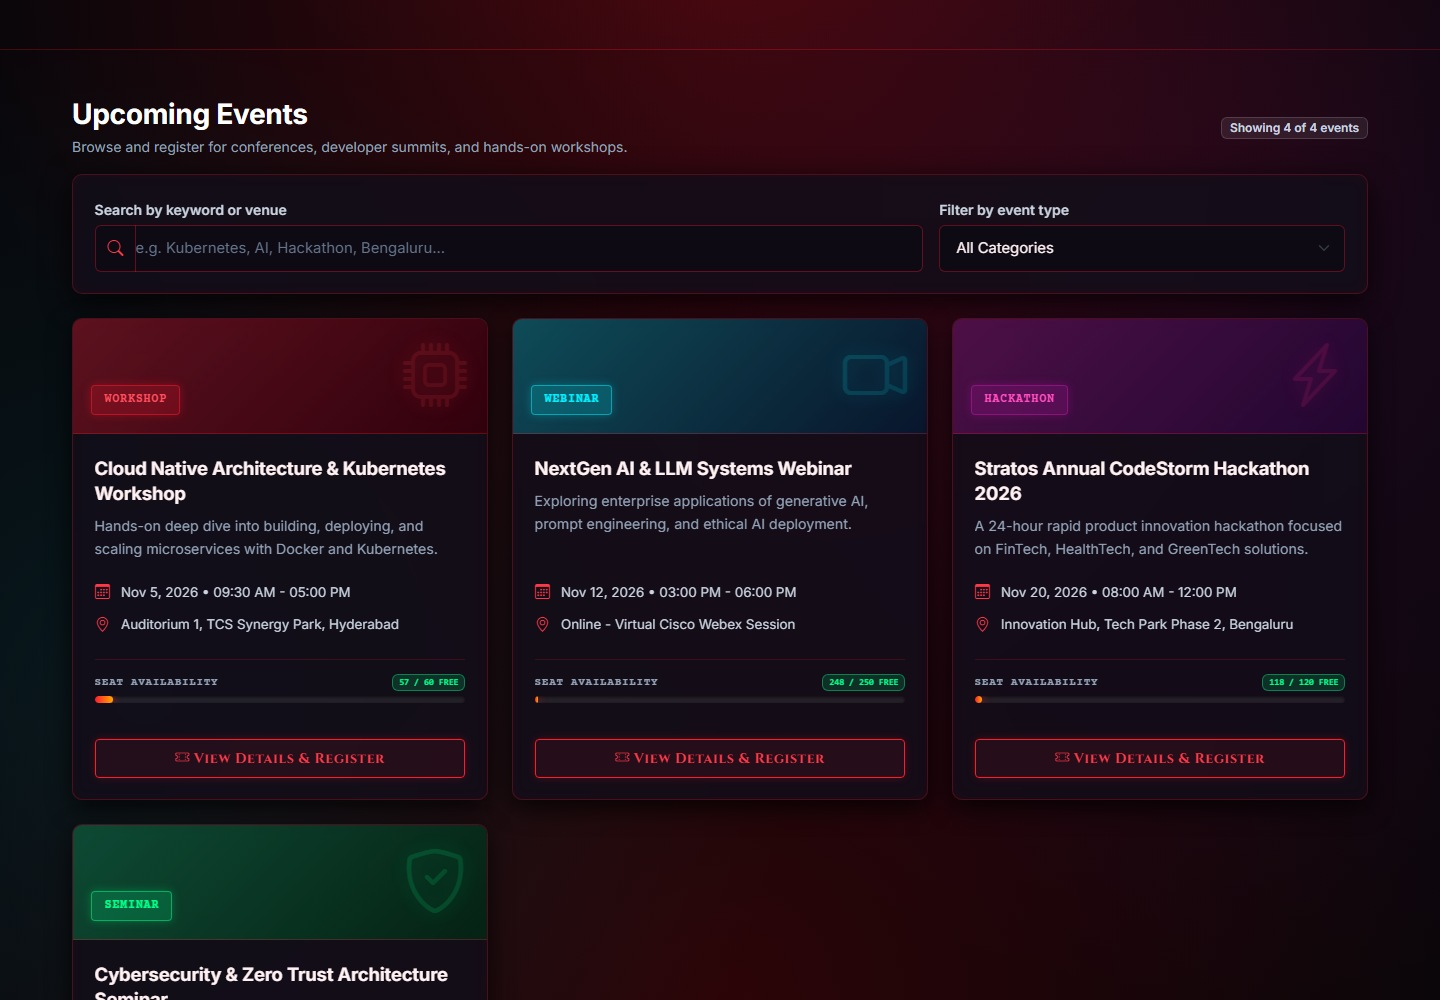
\includegraphics[width=0.92\textwidth]{screenshots/explore.png}
    \caption{Event Catalog with Search and Multi-Category Filters}
    \label{fig:explore}
\end{figure}

\subsection*{3. Event Details and Dynamic Ticket Tier Allocations}
When opening an event, attendees review full specifications and select from available ticket tiers. The modal dynamically renders live remaining seats (e.g., \textit{14 left}, \textit{8 left}), disabled \textit{Sold Out} badges, or \textit{Not Offered} indicators.

\begin{figure}[H]
    \centering
    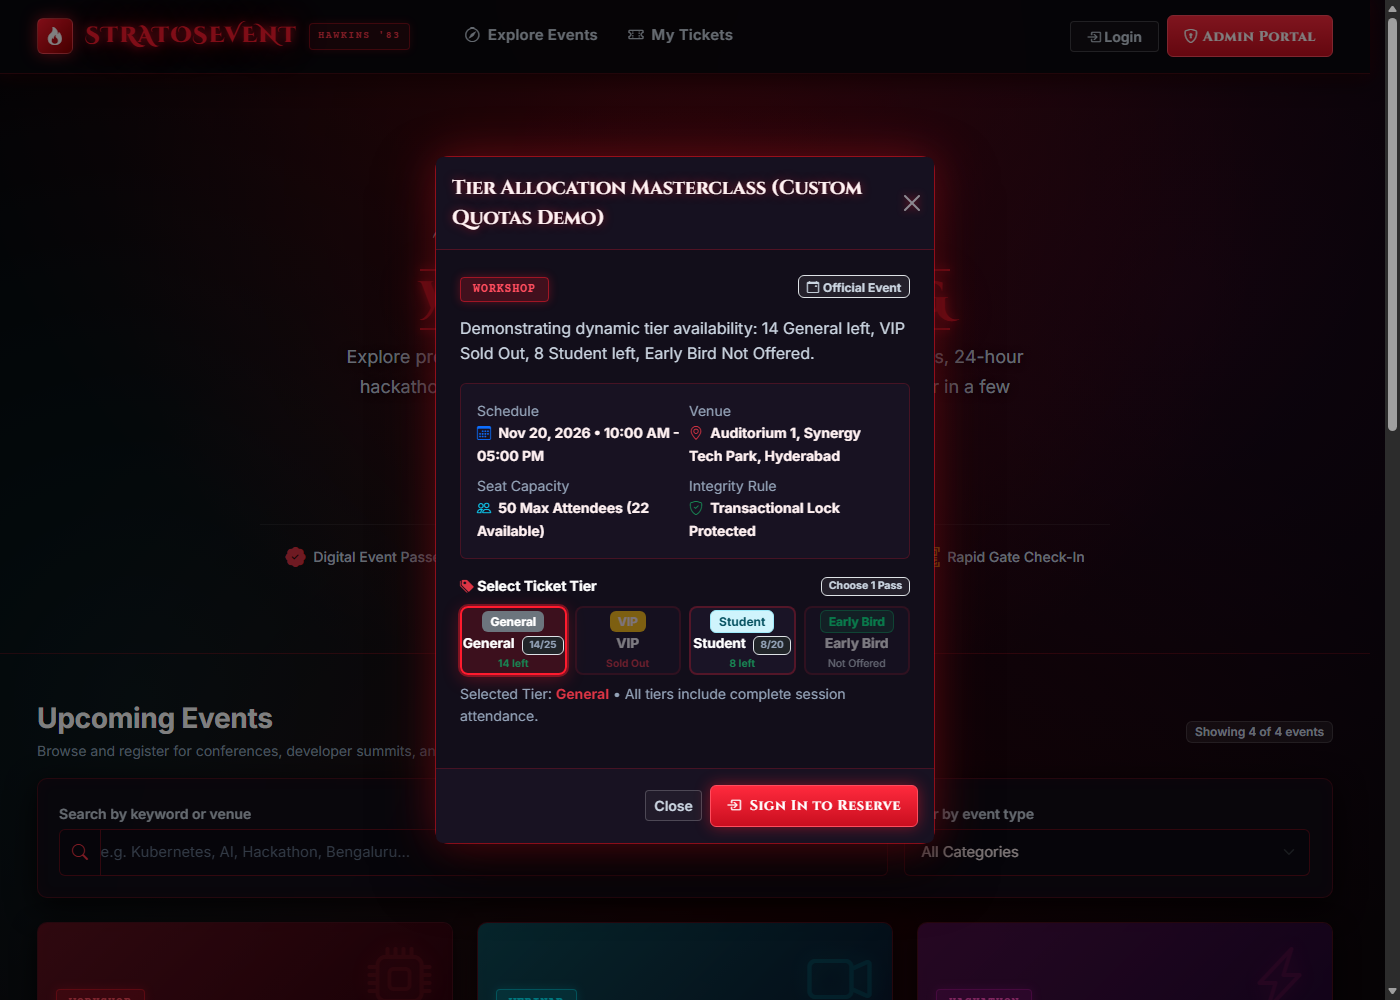
\includegraphics[width=0.88\textwidth]{screenshots/event-details.png}
    \caption{Event Modal with Dynamic Ticket Tier Availability}
    \label{fig:eventdetails}
\end{figure}

\subsection*{4. Clean Account Authentication (Sign In and Registration)}
A streamlined authentication modal provides clear email and password inputs without demo clutter, adhering to production event platform UX patterns.

\begin{figure}[H]
    \centering
    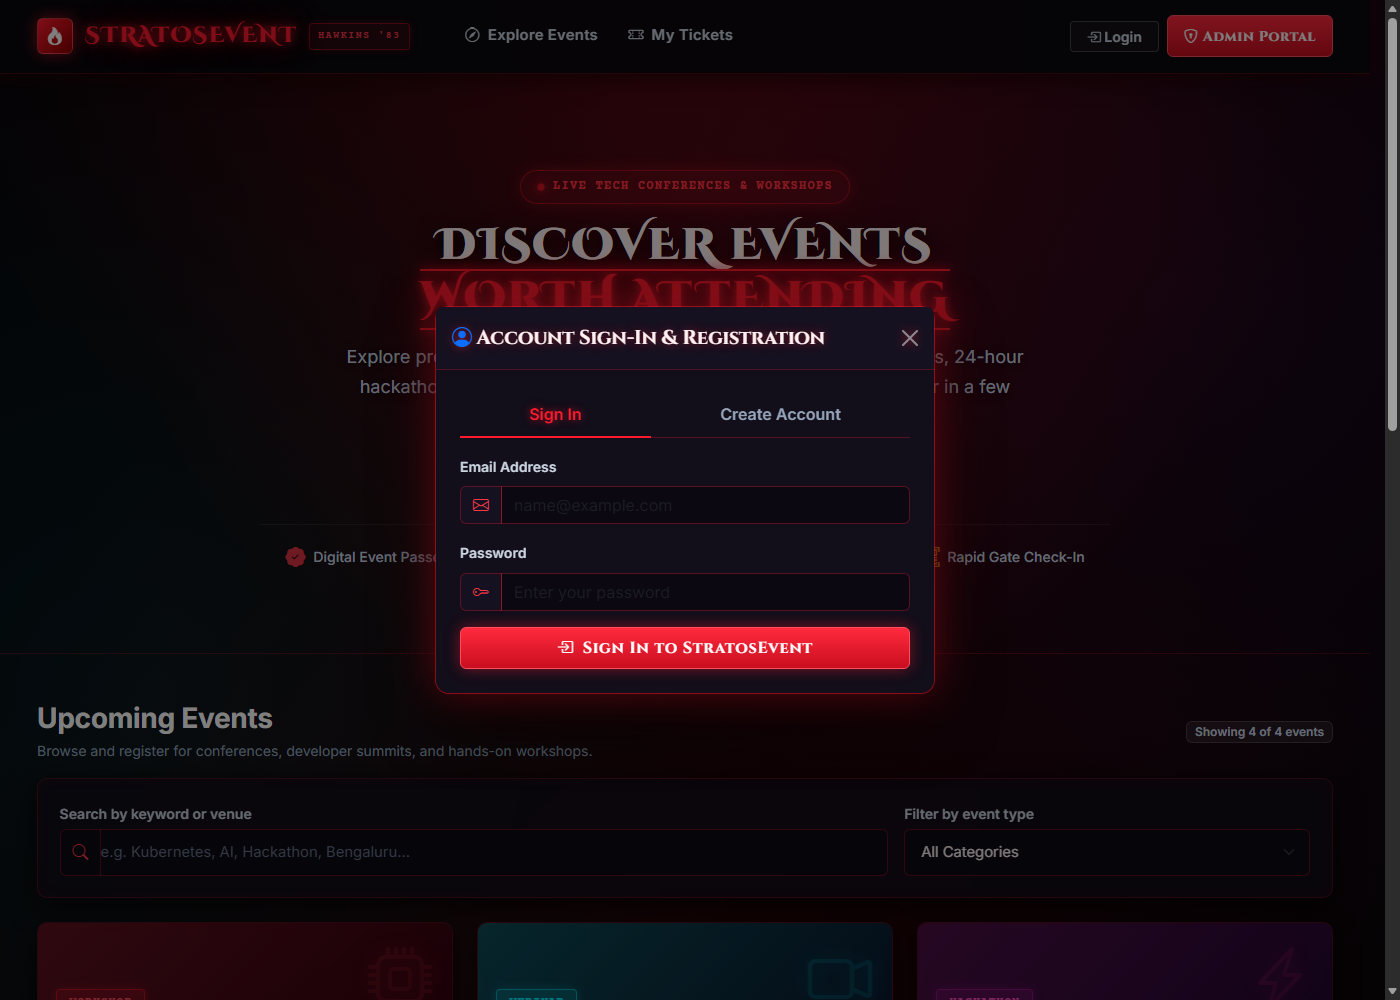
\includegraphics[width=0.75\textwidth]{screenshots/login.png}
    \caption{Participant and Administrator Sign-In Modal}
    \label{fig:login}
\end{figure}

\begin{figure}[H]
    \centering
    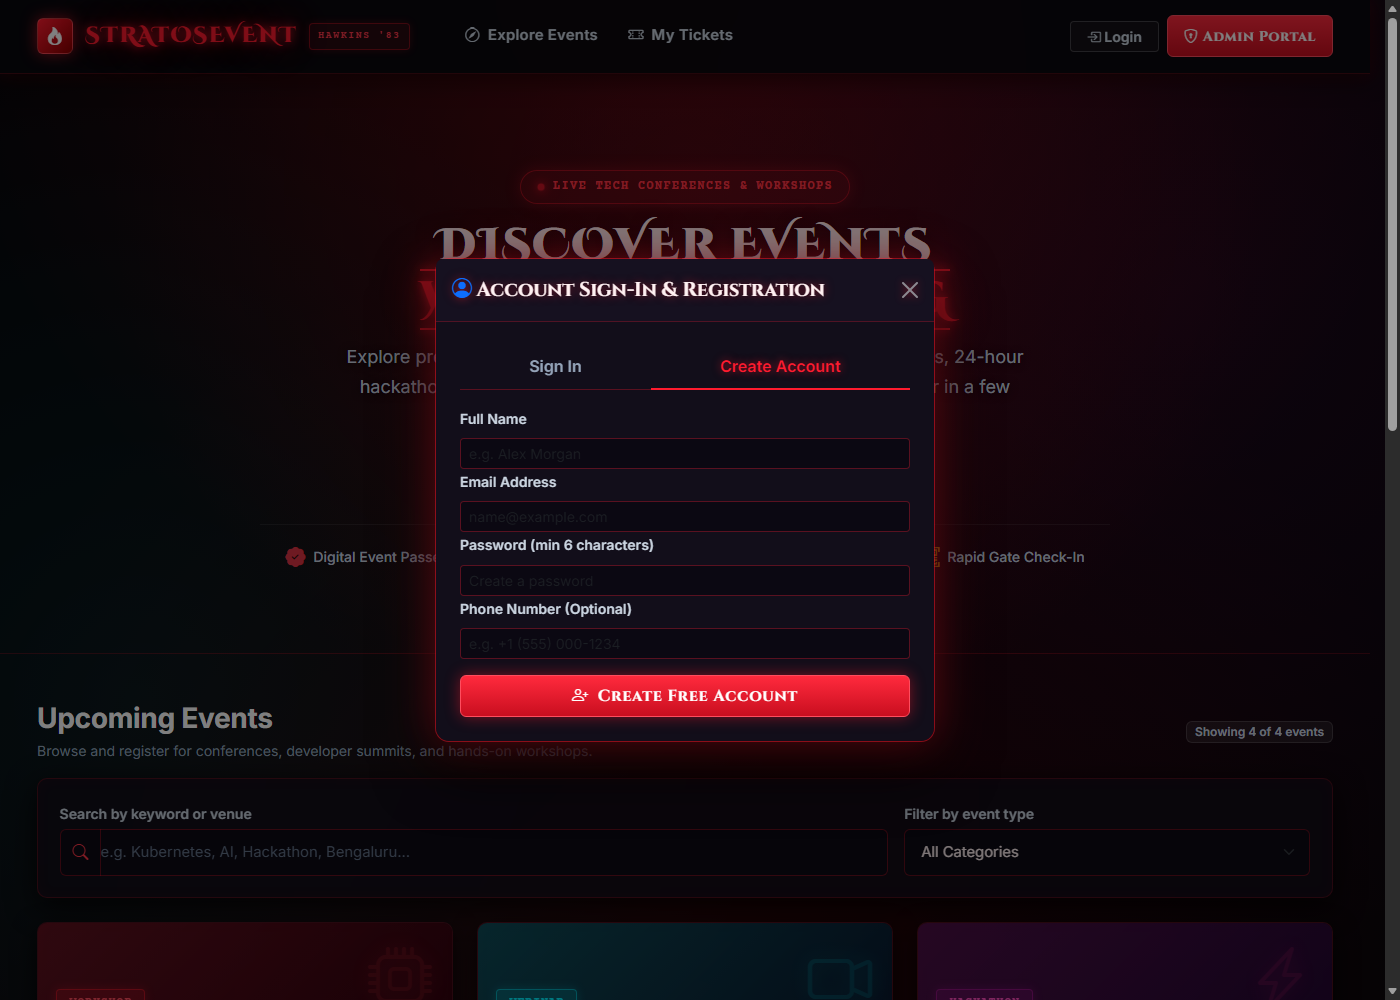
\includegraphics[width=0.75\textwidth]{screenshots/register.png}
    \caption{New Attendee Account Registration Modal}
    \label{fig:register}
\end{figure}

\subsection*{5. Confirmed Digital Ticket Pass}
Upon successful atomic reservation, the system renders an official booking pass complete with confirmed badge, prominent Ticket Tier badge, unique ticket code, and attendee identity.

\begin{figure}[H]
    \centering
    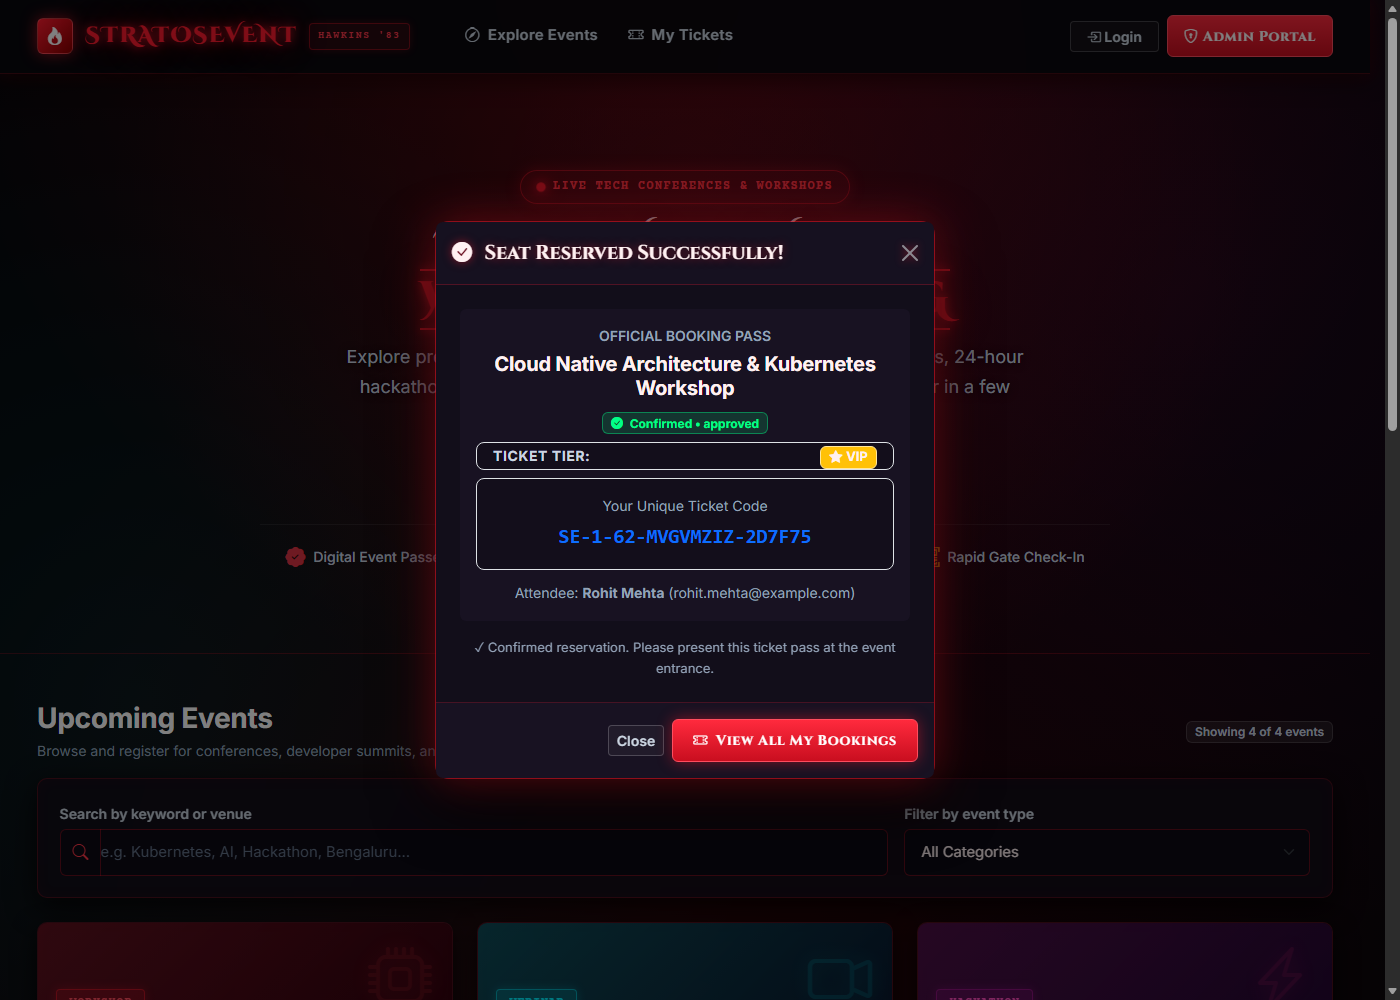
\includegraphics[width=0.82\textwidth]{screenshots/booking-confirmation.png}
    \caption{Official Verified Digital Ticket Pass}
    \label{fig:confirmation}
\end{figure}

\subsection*{6. Attendee Self-Service Portal (My Tickets and Passes)}
Participants can inspect all active and past registrations in a centralized dashboard, displaying ticket codes, tier badges, statuses, and one-click cancellation.

\begin{figure}[H]
    \centering
    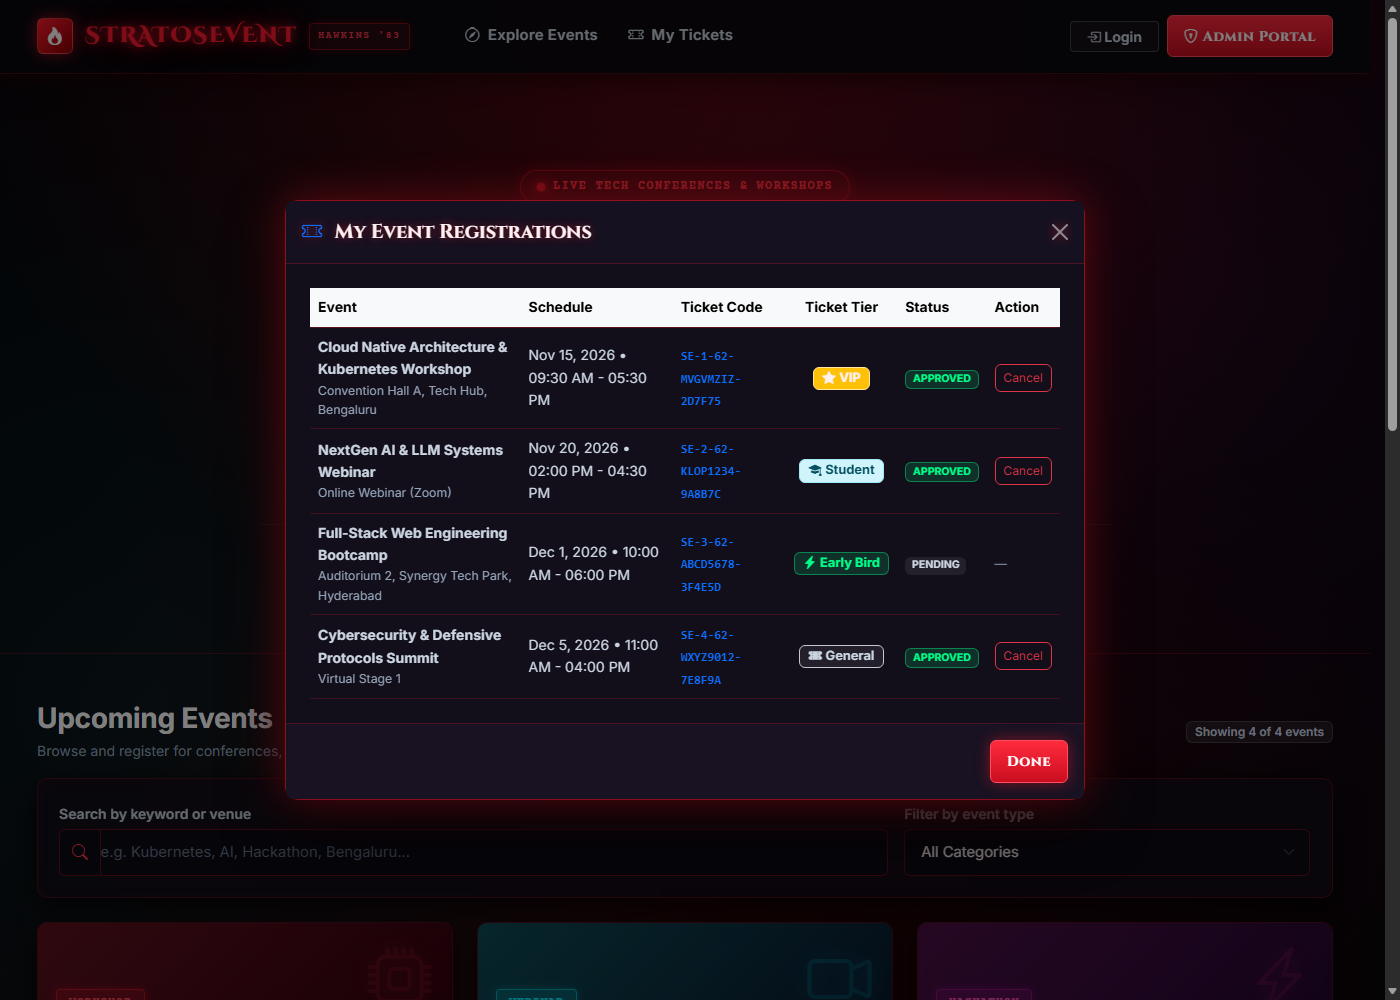
\includegraphics[width=0.92\textwidth]{screenshots/my-bookings.png}
    \caption{Attendee Self-Service Portal (My Tickets and Passes)}
    \label{fig:mybookings}
\end{figure}

\subsection*{7. Administrator Console - Registration Moderation}
Event coordinators review attendee rosters, filter by event or ticket tier, and perform real-time status transitions (Approve or Reject).

\begin{figure}[H]
    \centering
    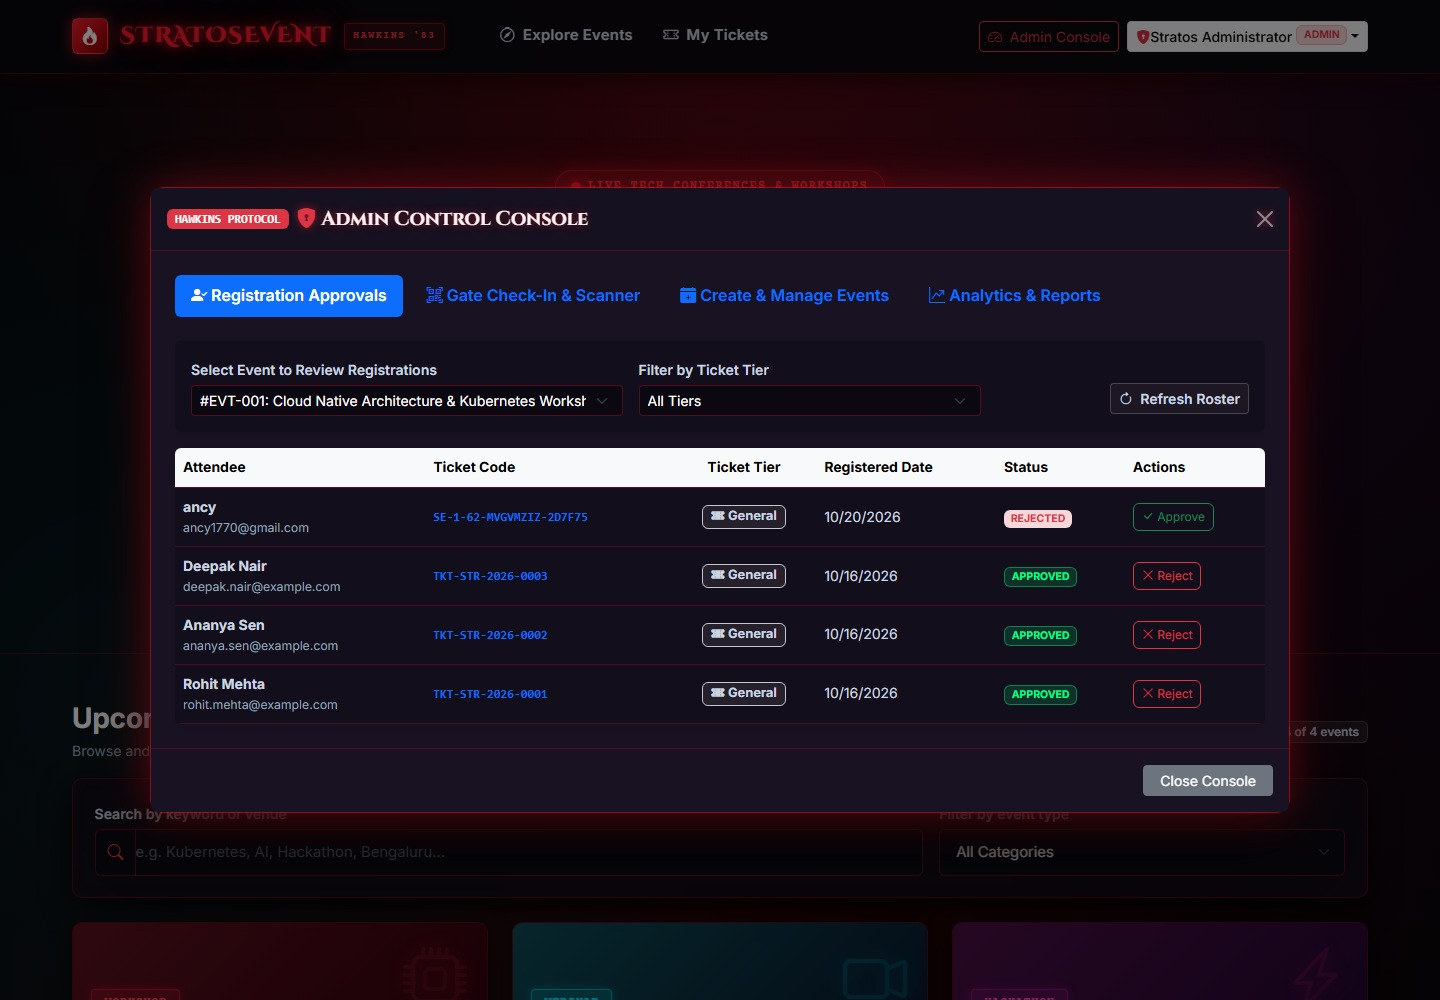
\includegraphics[width=0.92\textwidth]{screenshots/organizer-dashboard.png}
    \caption{Admin Control Console: Registration Approvals and Moderation}
    \label{fig:moderation}
\end{figure}

\subsection*{8. Administrator Console - Publish Event with Tier Seat Allocations}
Organizers configure upcoming events with custom seat capacities across General, VIP, Student, and Early Bird tiers, supported by live allocation counters and auto-distribution.

\begin{figure}[H]
    \centering
    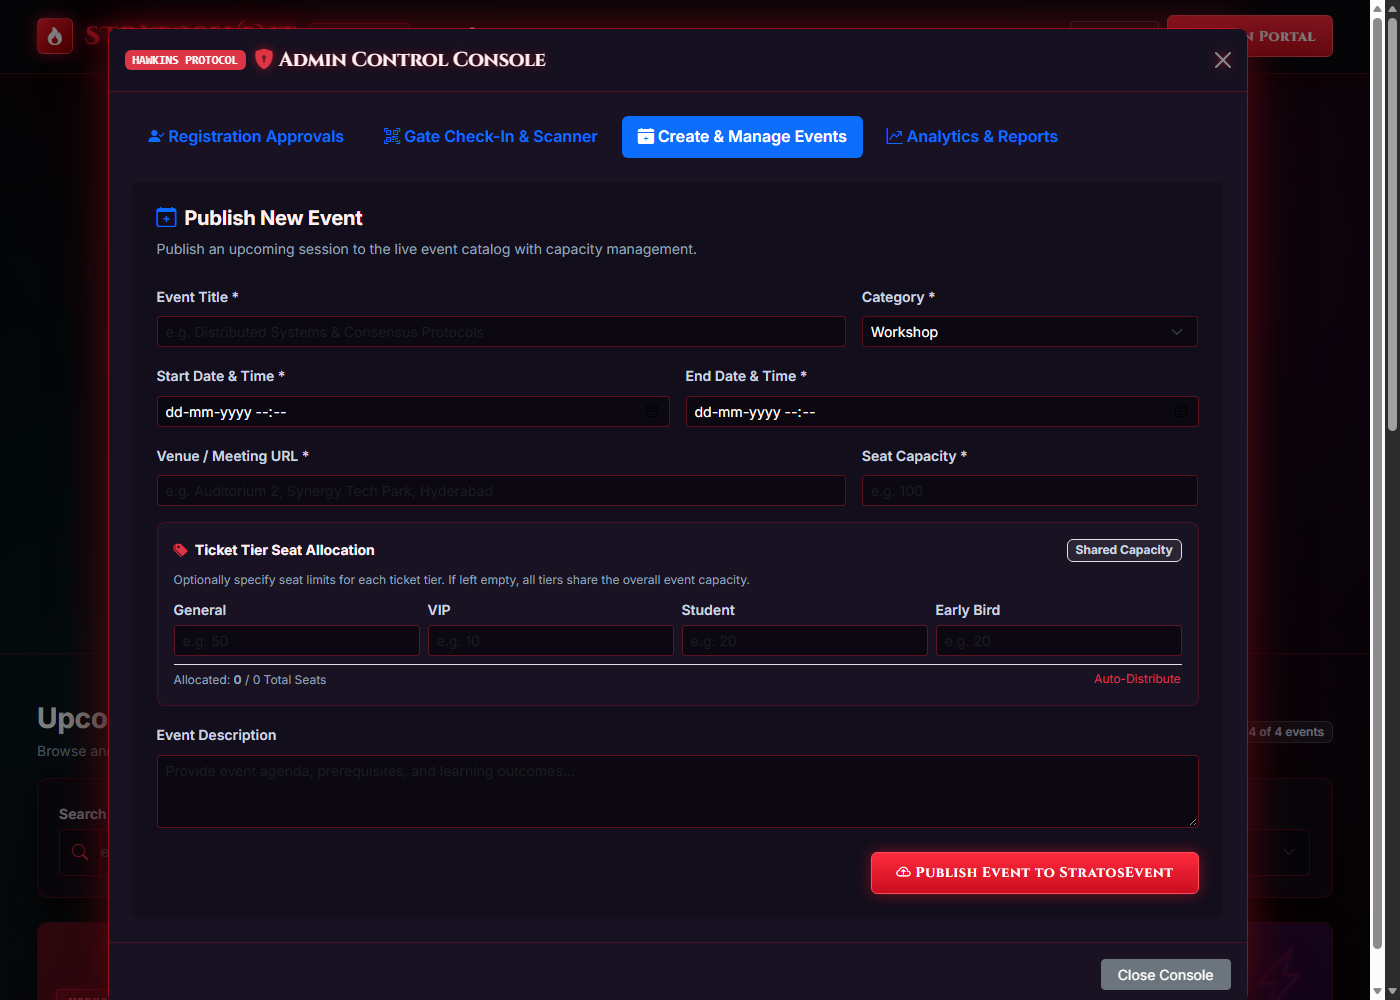
\includegraphics[width=0.88\textwidth]{screenshots/create-event.png}
    \caption{Admin Console: Publish New Event with Ticket Tier Allocations}
    \label{fig:createevent}
\end{figure}

\subsection*{9. Administrator Console - Gate Check-In Scanner}
Venue staff enter or scan attendee ticket codes at the entrance. The system verifies ticket validity in real time and records admission, rejecting duplicate check-ins.

\begin{figure}[H]
    \centering
    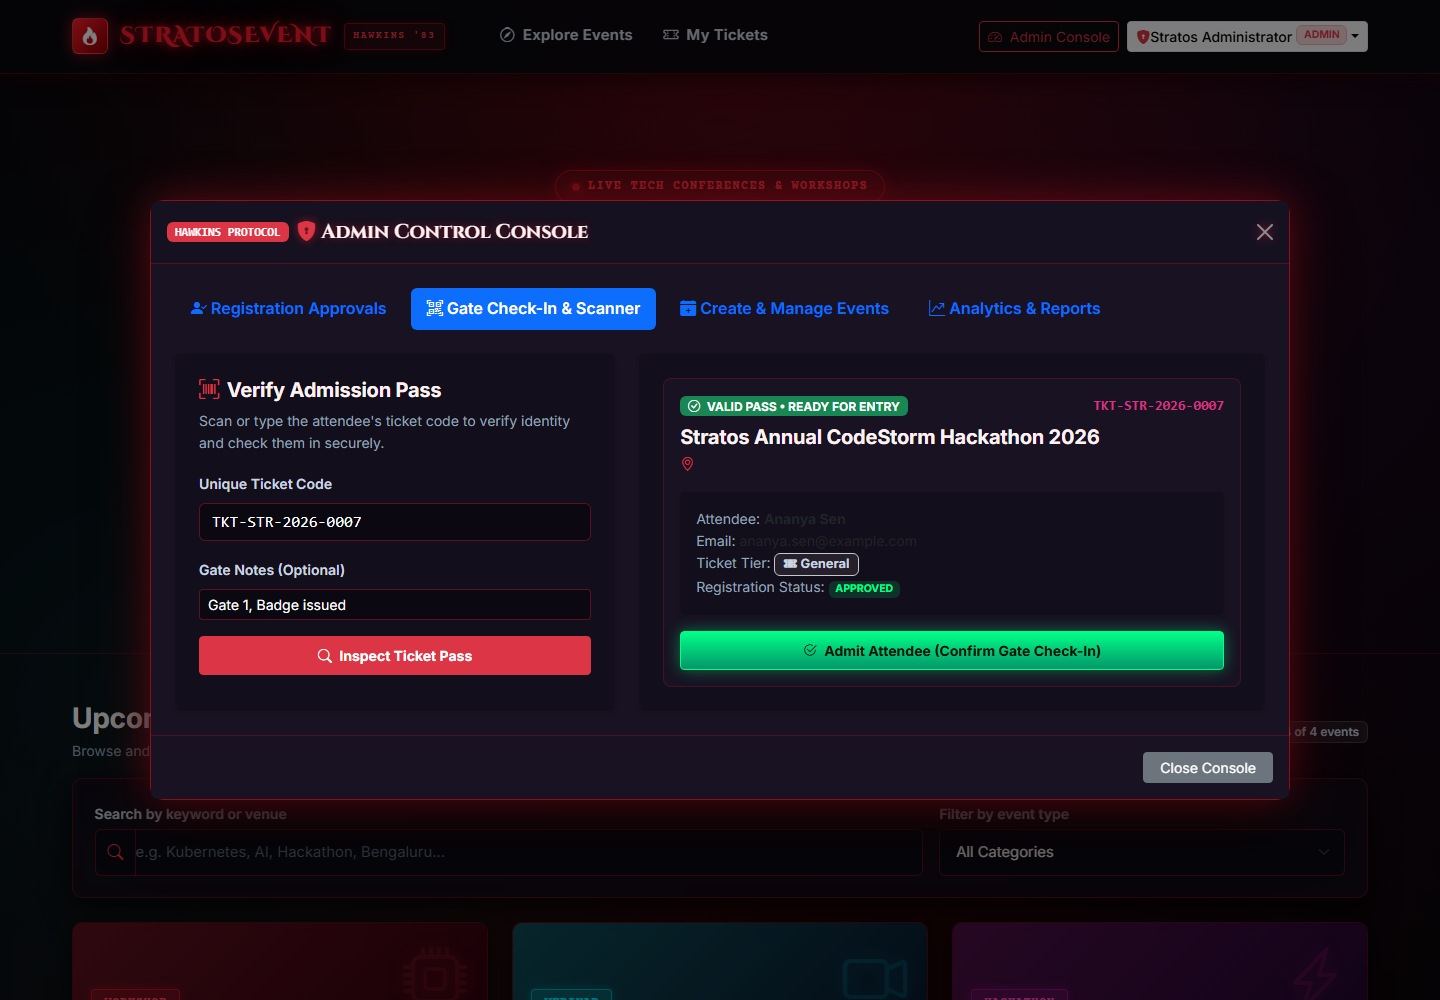
\includegraphics[width=0.88\textwidth]{screenshots/gate-scanner.png}
    \caption{Admin Console: Gate Check-In and Scanner Terminal}
    \label{fig:scanner}
\end{figure}

\subsection*{10. Administrator Console - Executive Analytics and CSV Export}
Provides leadership with real-time KPI metrics, attendance confirmation ratios, capacity gauges, and authorized one-click CSV roster export.

\begin{figure}[H]
    \centering
    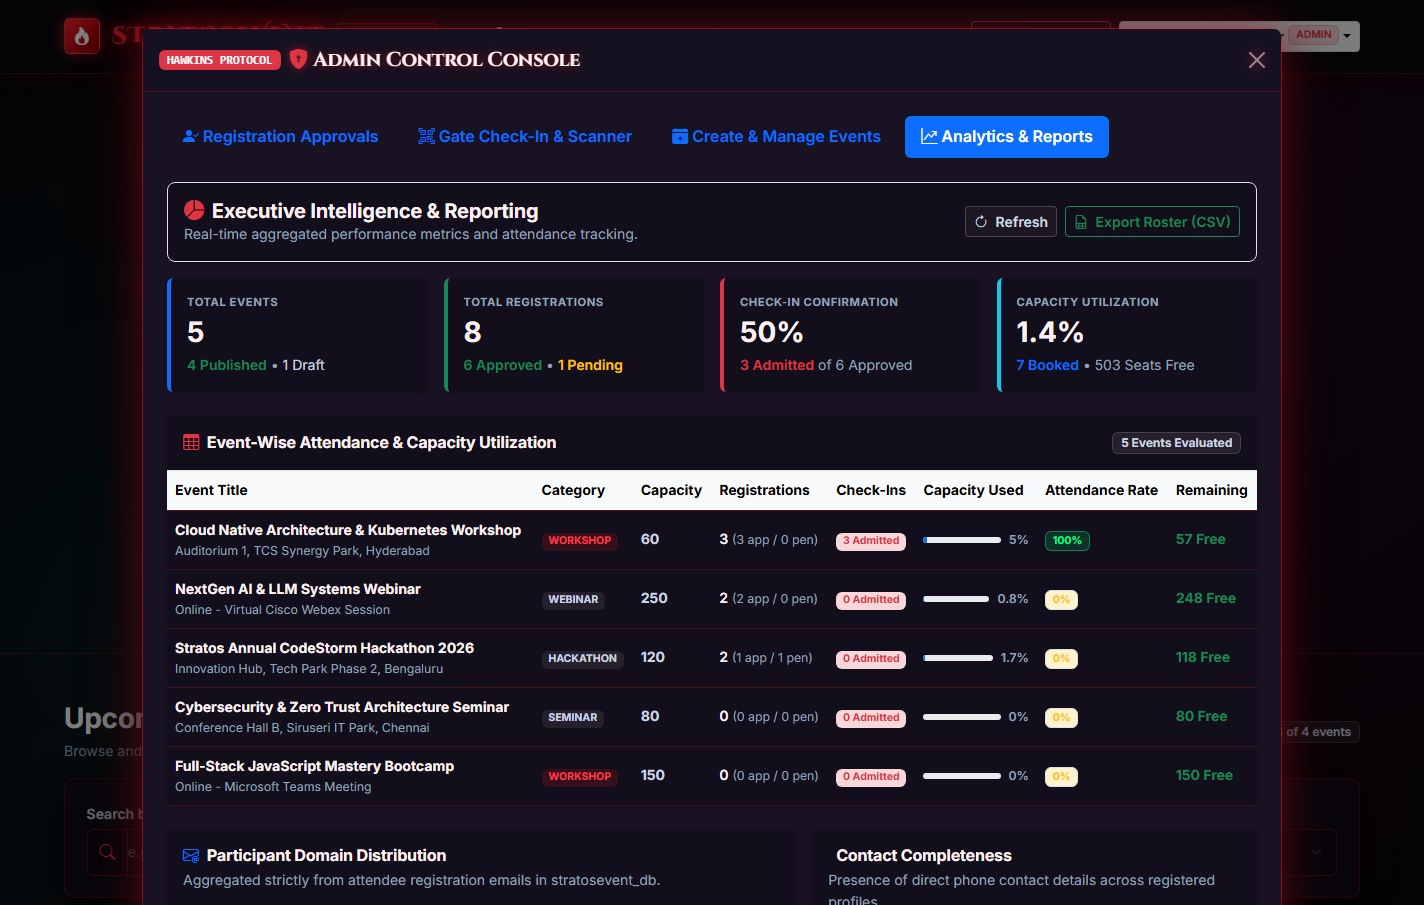
\includegraphics[width=0.92\textwidth]{screenshots/admin-dashboard.png}
    \caption{Admin Console: Executive Analytics and Business Intelligence}
    \label{fig:analytics}
\end{figure}

% ==========================================
% 10. CHALLENGES AND OPPORTUNITIES
% ==========================================
\newpage
\section*{{\color{TitleBlue}\bfseries
\fontsize{18}{22}\selectfont Challenges \& Opportunities}}
\addcontentsline{toc}{section}{Challenges \& Opportunities}

\subsection*{Technical Challenges Overcome}
\begin{enumerate}[leftmargin=*]
    \item \textbf{Eliminating Concurrency Race Conditions Under High Booking Load:} In high-demand scenarios, multiple HTTP requests attempt to reserve the final remaining seat simultaneously. We resolved this by wrapping reservation logic inside an explicit transaction with InnoDB row-level locking (\texttt{SELECT capacity, registered\_count FROM events WHERE id = ? FOR UPDATE}). The database serializes simultaneous requests, ensuring that exactly one user receives HTTP 201 Created while concurrent requests receive HTTP 409 Conflict (\texttt{CAPACITY\_REACHED}).
    \item \textbf{Mitigating Privilege Escalation (CWE-269):} To prevent malicious clients from granting themselves administrator rights by injecting \texttt{\{ "role": "admin" \}} during registration, the authentication controller strictly overrides payload roles, hardcoding public registrations to \texttt{'participant'}. Furthermore, administrative routes extract identity and role strictly from cryptographically verified JWT tokens.
    \item \textbf{Preventing CSV Formula Injection (CWE-1236):} Exporting attendee rosters to CSV presents security risks if user names begin with formula triggers (\texttt{=}, \texttt{+}, \texttt{-}, \texttt{@}). We implemented a sanitization helper (\texttt{escapeCSV}) that prefixes formula characters with a tab character and wraps values in double quotes, neutralizing spreadsheet execution.
    \item \textbf{Zero-Build Responsive Layout Without Viewport Overflow:} Developing a rich aesthetic while maintaining zero horizontal overflow across 375px mobile viewports required disciplined CSS architecture with CSS variables, \texttt{box-sizing: border-box}, and Bootstrap grid breakpoints.
\end{enumerate}

\subsection*{Opportunities for Future Expansion}
\begin{itemize}[leftmargin=*]
    \item \textbf{Optical QR Camera Scanner Integration:} Integrate the HTML5 WebRTC Camera API to allow gatekeepers to scan attendee QR codes directly through phone or tablet cameras without manual typing.
    \item \textbf{Automated Email/SMS Dispatch:} Integrate transactional email services (SendGrid / AWS SES) to dispatch PDF tickets and calendar invites upon registration approval.
    \item \textbf{Payment Gateway Webhooks:} Incorporate Stripe or Razorpay webhooks to support paid ticketing tiers alongside institutional complimentary passes.
\end{itemize}

% ==========================================
% 11. REFLECTIONS ON THE PROJECT
% ==========================================
\newpage
\section*{{\color{TitleBlue}\bfseries
\fontsize{18}{22}\selectfont Reflections on the Project}}
\addcontentsline{toc}{section}{Reflections on the Project}

\justifying

Building StratosEvent provided significant professional insights into modern full-stack software development:

\begin{itemize}[leftmargin=*]
    \item \textbf{Product-First Mindset over Academic Demonstrations:} Early iterations focused on explaining architectural features on the homepage. Transitioning to a discovery-first user experience—mirroring Eventbrite and Meetup—demonstrated that users prioritize intuitive event discovery, ticket selection, and clear registration over technical expositions.
    \item \textbf{The Critical Role of Database Concurrency:} Writing application-level checks (e.g., \texttt{if (registered < capacity)}) is fundamentally insufficient in multi-user web environments. True data consistency requires mastering relational database locking primitives, transaction boundaries, and isolation levels.
    \item \textbf{Simplicity and Performance with Native Web Standards:} Modern web standards (semantic HTML5, ES6+, CSS variables) provide exceptional developer velocity and high-performance user experiences without the bloat and fragility of complex frontend build pipelines.
    \item \textbf{Automated Testing as an Engineering Foundation:} Maintaining a suite of 59 unit/integration tests and 26 end-to-end flows provided continuous confidence during refactoring, ensuring zero regressions and 100\% data integrity.
\end{itemize}

% ==========================================
% 12. RECOMMENDATIONS
% ==========================================
\newpage
\section*{{\color{TitleBlue}\bfseries
\fontsize{18}{22}\selectfont Recommendations}}
\addcontentsline{toc}{section}{Recommendations}

\justifying

Based on the development and validation of StratosEvent, the following recommendations are offered for deploying transactional ticketing platforms:

\begin{enumerate}[leftmargin=*]
    \item \textbf{Enforce Row-Level Locking at the Database Engine:} Always utilize \texttt{SELECT ... FOR UPDATE} inside database transactions when managing constrained inventories. Never rely on in-memory counters or asynchronous read-then-write patterns.
    \item \textbf{Adopt Layered Defense Against Privilege Escalation:} Never trust user-supplied roles in registration payloads. Strictly bind user privileges to server-side cryptographic tokens (JWT) and evaluate role claims in centralized middleware.
    \item \textbf{Implement Compound Unique Constraints:} Back application validation with compound unique keys (e.g., \texttt{UNIQUE(user\_id, event\_id)}) to guarantee database-level prevention of duplicate bookings.
    \item \textbf{Sanitize All Administrative Data Exports:} Whenever generating CSV or Excel exports containing user-supplied input, neutralize formula trigger characters (\texttt{=}, \texttt{@}, \texttt{+}, \texttt{-}) to protect corporate users from spreadsheet malware.
    \item \textbf{Conduct Automated Concurrency Testing:} Include automated race-condition tests (e.g., simultaneous \texttt{Promise.all} requests competing for a single seat) in the continuous integration pipeline to verify capacity limits before deployment.
\end{enumerate}

% ==========================================
% 13. CONCLUSION
% ==========================================
\newpage
\section*{{\color{TitleBlue}\bfseries
\fontsize{18}{22}\selectfont Conclusion}}
\addcontentsline{toc}{section}{Conclusion}

\justifying

The \textbf{StratosEvent} platform successfully delivers a full-stack, enterprise-grade event management, dynamic registration, and real-time attendance verification system. By prioritizing an attendee-focused discovery experience and reinforcing every booking operation with atomic InnoDB row locking, the platform addresses and eliminates the systemic vulnerabilities of traditional event management systems.

All project milestones and architectural requirements have been met and verified:
\begin{itemize}[leftmargin=*]
    \item \textbf{Functional Completeness:} Comprehensive implementation of event discovery, per-tier seat allocation, atomic booking, digital pass issuance, self-service cancellation, administrator moderation, gate attendance scanning, and business intelligence reporting.
    \item \textbf{High Quality \& Security:} Mitigated CWE-269 privilege escalation, implemented HS256 JWT authentication, neutralized CWE-1236 CSV injection, and verified password security with bcrypt.
    \item \textbf{Verified Reliability:} Achieved a \textbf{100\% test pass rate across 59 automated test cases} in \texttt{backend/tests/api.test.js} and \textbf{26 end-to-end integration flows} in \texttt{backend/tests/e2e\_verification.js}.
    \item \textbf{Production-Ready Codebase:} Zero build bloat, clean directory organization, native Node.js runtime compatibility, and verified cross-device responsiveness.
\end{itemize}

StratosEvent represents a robust, scalable, and secure solution ready for real-world institutional and corporate deployment.

% ==========================================
% 14. ENHANCEMENT SCOPE
% ==========================================
\newpage
\section*{{\color{TitleBlue}\bfseries
\fontsize{18}{22}\selectfont Enhancement Scope}}
\addcontentsline{toc}{section}{Enhancement Scope}

\justifying

Future iterations of StratosEvent can build upon this solid architectural foundation with several planned enhancements:

\begin{itemize}[leftmargin=*]
    \item \textbf{Payment Gateway Webhooks:} Integration of Stripe, Razorpay, or PayPal webhook endpoints to support real-time paid ticket tier checkout and automated refund handling.
    \item \textbf{Automated Waitlist Promotion:} When an approved registration is cancelled, automatically promote the oldest pending registration to confirmed status and notify the attendee via email.
    \item \textbf{Multi-Tenancy Support:} Extend the database schema to support multiple independent organizations, each managing their own events, organizers, attendees, and custom subdomains.
    \item \textbf{Calendar Integration:} Provide one-click \texttt{.ics} calendar subscription feeds and Google Calendar / Outlook integration for registered attendees.
    \item \textbf{Progressive Web App (PWA):} Add service workers and a web manifest to enable offline ticket access and native-like installation on mobile home screens.
\end{itemize}

% ==========================================
% 15. LINK TO CODE AND EXECUTABLE FILE
% ==========================================
\newpage
\section*{{\color{TitleBlue}\bfseries
\fontsize{18}{22}\selectfont Link to Code and Executable File}}
\addcontentsline{toc}{section}{Link to Code and Executable File}

\vspace{0.10in}

\noindent
\textbf{1. Source Code Repository}

The complete source code, database migrations, documentation, and test suites for StratosEvent are maintained in the project repository:

\begin{center}
\href{https://github.com/stratosevent/stratosevent}
{\textbf{StratosEvent - Project Repository (GitHub)}}
\end{center}

\vspace{0.15in}
\noindent
\textbf{2. Local Project Execution (Visual Studio Code)}

StratosEvent is engineered as a zero-build, native full-stack web application. It runs locally using Visual Studio Code on Windows, macOS, or Linux:

\begin{enumerate}[leftmargin=*]
    \item \textbf{Prerequisites:}
    \begin{itemize}
        \item Node.js (v18.x or v20.x LTS)
        \item MySQL Server 8.0+ running locally on port 3306 with database \texttt{stratosevent\_db}
    \end{itemize}
    \item \textbf{Environment Configuration:} Configure \texttt{backend/.env}:
    \begin{verbatim}
    PORT=5000
    NODE_ENV=development
    DB_HOST=localhost
    DB_PORT=3306
    DB_USER=root
    DB_PASSWORD=YourPassword
    DB_NAME=stratosevent_db
    JWT_SECRET=your_super_secret_jwt_key_2026
    \end{verbatim}
    \item \textbf{One-Click Launch in VS Code:}
    \begin{itemize}
        \item Press \textbf{F5} to start the backend server via the pre-configured VS Code debug launch task (\textit{StratosEvent Backend Server (Port 5000)}).
        \item Open a terminal and run the frontend server: \texttt{npx serve frontend -l 3000}.
        \item Open \texttt{http://localhost:3000} in any browser.
    \end{itemize}
    \item \textbf{Run Automated Test Suites:}
    \begin{verbatim}
    cd backend
    node --test tests/api.test.js
    node tests/e2e_verification.js
    \end{verbatim}
\end{enumerate}

% ==========================================
% 16. RESEARCH QUESTIONS AND RESPONSES
% ==========================================
\newpage
\section*{{\color{TitleBlue}\bfseries
\fontsize{18}{22}\selectfont Research Questions and Responses}}
\addcontentsline{toc}{section}{Research Questions and Responses}

\subsection*{Research Question 1}
\textbf{How can a web application completely eliminate race conditions and overbooking when multiple users book the final seat simultaneously?}

\textbf{Response:}
Traditional web applications read current attendee counts and execute an insert in separate asynchronous operations. Under high traffic, concurrent requests read the same available seat count before any insert completes, resulting in overbooking. StratosEvent eliminates this by wrapping the availability check and registration insertion inside an isolated InnoDB transaction with pessimistic row-level locking (\texttt{SELECT capacity, registered\_count FROM events WHERE id = ? FOR UPDATE}). The database engine locks the event row, serializing all concurrent booking requests. Subsequent transactions wait until the active transaction commits or rolls back, guaranteeing zero overbooking.

\subsection*{Research Question 2}
\textbf{How can a public registration system prevent privilege escalation attacks without manual verification?}

\textbf{Response:}
Many applications accept JSON payloads containing a \texttt{"role"} field. If client input is passed directly to database insert statements, malicious users can register as administrators. StratosEvent prevents privilege escalation by hardcoding the user role to \texttt{'participant'} within the public registration controller, completely ignoring any \texttt{role} field supplied in the request body. Administrative accounts are seeded securely through protected server-side scripts, and all administrative endpoints evaluate permissions strictly against verified, tamper-proof JWT claims.

\subsection*{Research Question 3}
\textbf{How does granular per-tier seat allocation impact database design and booking validation?}

\textbf{Response:}
Rather than treating an event as a single homogeneous pool, StratosEvent stores dedicated capacity columns (\texttt{capacity\_general}, \texttt{capacity\_vip}, \texttt{capacity\_student}, \texttt{capacity\_early\_bird}) on the \texttt{events} table. When creating an event, the validator ensures the sum of tier quotas equals total event capacity. During registration, the system counts active bookings for the requested tier inside an atomic lock; if the tier quota is reached, it returns \texttt{409 TIER\_CAPACITY\_REACHED}, preventing tier overbooking while keeping unexhausted tiers open.

\subsection*{Research Question 4}
\textbf{What security measures are required when exporting attendee rosters to CSV format?}

\textbf{Response:}
CSV export endpoints are susceptible to Formula Injection (CWE-1236). If an attendee registers with a name beginning with formula triggers (such as \texttt{=cmd|' /C calc'!A0}), spreadsheet software executes arbitrary system commands upon opening the file. StratosEvent implements strict formula neutralization: any field starting with \texttt{=}, \texttt{+}, \texttt{-}, or \texttt{@} is automatically prefixed with a tab character (\texttt{\textbackslash t}) and enclosed in double quotes, neutralizing execution while preserving readable textual output.

\subsection*{Research Question 5}
\textbf{How can digital ticket passes be designed to prevent gate-entry fraud and duplicate check-in?}

\textbf{Response:}
StratosEvent generates cryptographically unique ticket codes adhering to the structure \texttt{SE-[EventID]-[UserID]-[TimestampHash]-[RandomSalt]} upon registration approval. At the venue entrance, staff query the verification endpoint (\texttt{GET /api/attendance/verify/:code}), which checks whether the ticket is approved and unredeemed. When check-in is submitted, a record is inserted into the \texttt{attendance} table, which enforces a unique constraint on \texttt{registration\_id}. Any subsequent check-in attempt immediately fails with \texttt{409 DUPLICATE\_CHECKIN}, preventing ticket pass reuse.

% ==========================================
% 17. REFERENCES
% ==========================================
\newpage
\section*{{\color{TitleBlue}\bfseries
\fontsize{18}{22}\selectfont References}}
\addcontentsline{toc}{section}{References}

\begin{enumerate}[leftmargin=*]
    \item \textbf{Fielding, R. T.} (2000). \textit{Architectural Styles and the Design of Network-based Software Architectures}. Doctoral dissertation, University of California, Irvine.
    \item \textbf{Oracle Corporation.} (2024). \textit{MySQL 8.0 Reference Manual: InnoDB Locking and Transaction Model}. Oracle Documentation. \url{https://dev.mysql.com/doc/refman/8.0/en/innodb-locking.html}
    \item \textbf{Jones, M., Bradley, J., \& Sakimura, N.} (2015). \textit{JSON Web Token (JWT)}. RFC 7519, Internet Engineering Task Force (IETF). \url{https://datatracker.ietf.org/doc/html/rfc7519}
    \item \textbf{OWASP Foundation.} (2021). \textit{OWASP Top 10: Broken Access Control (CWE-269)}. Open Web Application Security Project. \url{https://owasp.org/Top10/A01_2021-Broken_Access_Control/}
    \item \textbf{OWASP Foundation.} (2023). \textit{CSV Injection Prevention Cheat Sheet (CWE-1236)}. OWASP Cheat Sheet Series. \url{https://cheatsheetseries.owasp.org/cheatsheets/CSV_Injection_Cheat_Sheet.html}
    \item \textbf{OpenJS Foundation.} (2024). \textit{Node.js v20.x Documentation: Test Runner and Asynchronous Operations}. Node.js Official Documentation. \url{https://nodejs.org/docs/latest-v20.x/api/}
    \item \textbf{Express.js Core Team.} (2024). \textit{Express 4.x API Reference: Routing and Middleware}. \url{https://expressjs.com/}
    \item \textbf{Bootstrap Team.} (2024). \textit{Bootstrap v5.3 Documentation: Responsive Breakpoints and Grid System}. \url{https://getbootstrap.com/docs/5.3/}
\end{enumerate}

\end{document}
